\documentclass[UTF8]{ctexart}
\usepackage{geometry}
\geometry{margin=1.5cm, vmargin={0pt,1cm}}
\setlength{\topmargin}{-1cm}
\setlength{\paperheight}{29.7cm}
\setlength{\textheight}{25.3cm}

% useful packages.
\usepackage{amsfonts}
\usepackage{amsmath}
\usepackage{amssymb}
\usepackage{amsthm}
\usepackage{enumerate}
\usepackage{graphicx}
\usepackage{multicol}
\usepackage{fancyhdr}
\usepackage{layout}
\usepackage{float}
\usepackage{listings}
\usepackage{xcolor}
\lstset{language=C++}
\setlength{\headheight}{13pt}  % 增加头部高度
\usepackage{float, caption}

% Listings setting for code formatting
\lstset{
    basicstyle=\ttfamily,
    keywordstyle=\color{blue},
    commentstyle=\color{gray},
    stringstyle=\color{red},
    breaklines=true,
    frame=single,
    numbers=left,
    numberstyle=\tiny,
    stepnumber=1,
    tabsize=4
}

% some common commands
\newcommand{\dif}{\mathrm{d}}
\newcommand{\avg}[1]{\left\langle #1 \right\rangle}
\newcommand{\difFrac}[2]{\frac{\dif #1}{\dif #2}}
\newcommand{\pdfFrac}[2]{\frac{\partial #1}{\partial #2}}
\newcommand{\OFL}{\mathrm{OFL}}
\newcommand{\UFL}{\mathrm{UFL}}
\newcommand{\fl}{\mathrm{fl}}
\newcommand{\op}{\odot}
\newcommand{\Eabs}{E_{\mathrm{abs}}}
\newcommand{\Erel}{E_{\mathrm{rel}}}

\begin{document}

\pagestyle{fancy}
\fancyhead{}
\lhead{陈梓锐}
\chead{22435036}
\rhead{Dec.15th, 2024}

\section*{内容}
\begin{enumerate}
    \item 在ppForm和BSpline格式下实现$\mathbb{S}_{1}^{0} $和$\mathbb{S}_{3}^{2} $。
    \item 在ppForm条件下推导（概述）并实现了三次样条函数$\mathbf{S}_{3}^{2}$:周期边界条件，自然边界条件，完全边界条件（任意节点）。
    \item 在BSpline条件下推导（概述）并实现了三次样条函数$\mathbf{S}_{3}^{2}$:周期边界条件，自然边界条件，完全边界条件（任意节点）。
    \item 验证在ppForm和BSpline条件下，三次样条函数$\mathbf{S}_{3}^{2}$是相同的(在problemA中验证了)。
    \item 验证了BSpline格式下支持任意阶任意节点的样条绘制。(任意阶只要给出合适的边界条件都可以获得良好的拟合曲线，
          任意节点在problemE中使用cumulative chordal length时已经验证)
    \item 实现平面上的样条曲线拟合。(problemE中的心形线与螺线)
    \item 实现球面上的样条曲线拟合。(problemE中的三维样条曲线)
    \item 实现了书上的问题。
\end{enumerate}

\section*{附加分数}
\begin{enumerate}
    \item 任意阶的样条曲线绘制。
    \item 更多例子验证。
\end{enumerate}

\section*{ppForm实现$\mathbb{S}_{1}^{0} $}
\subsection*{概述}
    因为$\mathbb{S}_{1}^{0} $的定义为分段线性函数，所以只需要对每个分段进行线形插值即可。
\subsection*{实现}
\begin{enumerate}
    \item 首先，在构造函数ppForm中加入一个bool型的参数表明此时构造的是线性样条。
    \begin{lstlisting}
    ppForm(const Function& f, double a, double b,int nodeCount, bool isLinear)
    : f(f), nodeCount(nodeCount);
    \end{lstlisting}
    \item 接下来，实现线性插值并返回插值结果。
    \begin{lstlisting}
    double LinearInterpolation(double x);
    \end{lstlisting}
\end{enumerate}

\section*{ppForm实现$\mathbb{S}_{3}^{2} $}
\subsection*{概述}
    想要实现$\mathbb{S}_{3}^{2} $，需要对每个分段线性函数进行三次样条插值。

    首先，我们记$S_{i}(x)$为函数在$x\in[x_{i},x_{i+1}]$处的插值函数，记$h_{i} = x_{i+1}-x_{i}$
    ,$S^{''}(x_{i}) = M_{i}$, $i = 0, 1,\cdots, n$。由于$S_{i}^{''}(x)$的线性性，我们有
    $$S_{i}^{''}(x) = \frac{x_{i+1} - x}{h_{i}} M_{i} + \frac{x - x_{i}}{h_{i}} M_{i+1}$$
    对上述等式两边做两次积分，我们有
    $$S_{i}(x) = \frac{(x_{i+1} - x)^{3}}{6h_{i}} M_{i} + \frac{(x - x_{i})^{3}}{6h_{i}} M_{i+1} +
        A_{i}(x - x_{i+1}) + B_{i}$$
    利用插值条件$S_{i}(x_{i}) = f_{i}$, $S_{i}(x_{i+1}) = f_{i+1}$，我们有
    $$A_{i} = \frac{f_{i+1} - f_{i}}{h_{i}} - \frac{h_{i}}{6}(M_{i+1} - M_{i})
        \ ,\ B_{i} = f_{i+1} - \frac{h_{i}^{2}}{6}M_{i+1}$$
    从而有，
    $$S_{i}(x) = \frac{(x_{i+1} - x)^{3}}{6h_{i}} M_{i} + \frac{(x - x_{i})^{3}}{6h_{i}} M_{i+1}
                + (f_{i} - \frac{M_{i}}{6}h_{i}^{2}) \frac{x_{i+1} - x}{h_{i}}
                + (f_{i+1} - \frac{M_{i+1}}{6}h_{i}^{2}) \frac{x - x_{i}}{h_{i}}$$
    接下来我们求解$M_{i}$即可确定三次样条函数的表达式，需要用到样条一阶导连续的性质。
    首先对$S_{i}(x)$求导，
    $$\S_{i}^{''}(x) = - \frac{(x_{i+1} - x)^{2}}{2h_{i}} M_{i} + \frac{(x - x_{i})^{2}}{2h_{i}} M_{i+1} 
                       + \frac{f_{i+1} - f_{i}}{h_{i}} + \frac{M_{i+1} - M_{i}}{6} h_{i} $$
    利用一阶导连续性，有
    $$\frac{h_{i}}{6}M_{i} + \frac{h_{i} + h_{i+1}}{3}M_{i+1} + \frac{h_{i+1}}{6}M_{i+2}
        = f[x_{i+1}, x_{i+2}] - f[x_{i}, x_{i+1}] $$
    上是两端同时除以$(h_{i+1}+h_{i})/6$，有
    $$\mu_{i+1}M_{i} + 2M_{i+1} + \lambda_{i+1}M_{i+2} = b_{i+1}$$
    其中，
    $$\mu_{i+1} = \frac{h_{i}}{h_{i} + h_{i+1}}, \lambda_{i+1} = \frac{h_{i+1}}{h_{i} + h_{i+1}}, 
        d_{i+1} = 6f[x_{i}, x_{i+1}, x_{i+2}]$$
    结合两个边界条件即可求出$M_{i}$。
\subsection*{实现}
\begin{enumerate}
    \item 首先，定义一个枚举类SplineType，用于表示使用三次样条的边界条件。
    \begin{lstlisting}
    enum class SplineType{
        Natural,
        Complete,
        Periodic
    };
    \end{lstlisting}

    \item 在构造函数中初始化插值点以及插值点的函数值。平均插值点和任意插值点调用不同的构造函数。
    \par 平均插值点和任意点的构造函数如下：
    \begin{lstlisting}
    ppForm(const Function& f, double a, double b,int nodeCount, SplineType splineType = SplineType:: Natural);
    ppForm(const Function& f, std::vector<double> nodes, SplineType splineType = SplineType:: Natural)
    \end{lstlisting}

    \item 进入useFunction函数，根据传入的枚举类型确定三次样条的边界条件。
    \begin{lstlisting}
    void useFunction()
    \end{lstlisting}

    \item 函数calMiu(int i)用于计算$\mu_{i}$，函数calNabuda(int i)用于计算$\lambda_{i}$。
    \begin{lstlisting}
    double calMiu(int i)；
    double calNabuda(int i);
    \end{lstlisting}

    \item 计算二阶差商$f[x_{i}, x_{i+1}]$和三阶差商$f[x_{i-1}, x_{i}, x_{i+1}]$。
    \begin{lstlisting}
    double calQuadraticDivided(int i)；
    double calCubicDivided(int i)；
    \end{lstlisting}

    \item 求解三对角矩阵的解。
    \begin{lstlisting}
    void caltridiagonal()；
    \end{lstlisting}

    \item 根据给定边界条件，调用相应的函数，完成矩阵方程组的初始化
    ，并调用caltridiagonal函数求解三对角矩阵的解，即$M_{i}$。
    \begin{lstlisting}
    void computeNaturalSpline();
    void computeCompleteSpline();
    void computePeriodicSpline();
    void caltridiagonal();
    \end{lstlisting}
    

    \item 最后，我们计算插值点的函数值。
    \begin{lstlisting}
    double getValue(double x);
    \end{lstlisting}
\end{enumerate}

\section*{BSpline}
\subsection*{概述}
    根据书上内容，只需写出BSpline基函数，求出基函数的系数，即可求出插值函数。
    \begin{align}
        &B_{i}^{k}(x) = \frac{x - t_{i-1}}{t_{i+k} - t_{i-1}}B_{i-1}^{k-1}(x) 
                       + \frac{t_{i+k-1} - x}{t_{i+k}-t_{i}}B_{i+1}^{k-1}(x), \\
        &B_{i}^{k} \geq 0, \quad x \in [t_{i-1}, t_{i+k}].
    \end{align}
    其中，$t_{i}$为节点，$k$为次数。

    由于BSpline基函数的支撑性，我们需要扩展插值点$\{x_{i}\}_{i=0}^{n}$为节点，使得基函数的支撑集包含插值点,
    记节点集合为$T = \{t_{0}, t_{1}, \cdots, t_{m}\}$。
    其中，$m = n + k, x_{i} = t_{i+k}$。

    考虑插值基函数的支撑性，在插值边界$x_{0} = t_{k}, x_{n} = t_{n+k}$处，
    \begin{center}  
        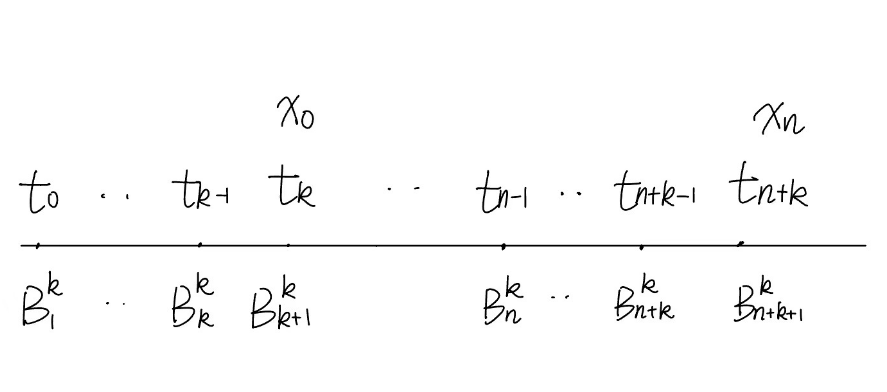
\includegraphics[scale=0.5]{zhicheng.png}
    \end{center}
    如图所示，$B_{k+1}^{k}(x_{0}) = 0, B_{n+k+1}^{k}(x_{n}) = 0$，
    所以对每个节点$x_{i}$,对其其作用的基函数有$B_{i-k+1}^{k}(x), B_{i-k+2}^{k}(x), \cdots, B_{i}^{k}(x)$。
    对于待拟合函数$f(x)$，我们可以将其表示为
    \begin{align}
        f(x) &= \sum_{i=1}^{m} P_{i}B_{i}^{k}(x),\\
        f(x_{j}) &= \sum_{i=1}^{m} P_{i}B_{i}^{k}(t_{j+k}) = \sum_{i=i-k+1}^{i} P_{i}B_{i}^{k}(t_{j+k}),\\
    \end{align}
    写成矩阵的形式即
    $$
    \begin{pmatrix}
        f(x_{0}) \\
        f(x_{1}) \\
        \vdots \\
        f(x_{n})
    \end{pmatrix}\begin{pmatrix}
        B_{1}^{k}(t_{k}) & B_{2}^{k}(t_{k}) & \cdots & B_{k}^{k}(t_{k}) & 0 & 0 \\
        0 & B_{2}^{k}(t_{k+1}) & \cdots & B_{k+1}^{k}(t_{k+1}) & 0 & 0 \\
        \vdots \\
        0 & \cdots & B_{n+1}^{k}(t_{n+k}) & B_{n+2}^{k}(t_{k}) & \cdots & B_{n+k}^{k}(t_{n+k}) \\
    \end{pmatrix} = \begin{pmatrix}
        P_{1} \\
        P_{2} \\
        \vdots \\
        P_{n+k}
    \end{pmatrix}
    $$
    显然系数矩阵是一个$(n+1) \times (n+k)$阶的矩阵，其中$P_{i}$为待拟合函数的系数，想要求解还需要提供$k-1$个边界条件。

    \subsubsection*{\textbf{$\mathbb{B} _{3}$}}
    考虑三次B样条的边界条件：自然，完全，周期。
    
    \begin{enumerate}
        \item 自然边界条件：$f^{''}(x_{0}) = f^{''}(x_{n}) = 0$。
        利用课本中的B样条导数公式和（3），当$k=3$时，有
        \begin{align}
            &f^{''}(x) = \sum_{j = 1}^{m} \left[\frac{6}{t_{j+2} - t_{j-1}}
                        (\frac{B_{j}^{1}(x)}{t_{j+1}-t_{j-1}} - \frac{B_{j+1}^{1}(x)}{t_{j+2}-t_{j}})
                        - \frac{6}{t_{j+3}-t_{j}}
                        (\frac{B_{j+1}^{1}(x)}{t_{j+2}-t_{j}} - \frac{B_{j+2}^{1}(x)}{t_{j+3}-t_{j+1}})P_{j}\right] \\
            & \\
            &B_{i}^{1}(x) = \left\{
                        \begin{array}{rl}
                        &\frac{x - t_{i-1}}{t_{i} - t_{i-1}}, \qquad x \in (t_{i-1}, t_{i}] \\
                        &\frac{t_{i+1} - x}{t_{i+1} - t_{i}}, \qquad x \in (t_{i}, t_{i+1}) \\
                        &0, \qquad otherwise \\
                        \end{array}
                        \right.
        \end{align}
        分别带入$x_{0}, x_{n}$, 即可得到边界条件。

        \item 完全边界条件：$f^{'}(x_{0}) = f^{'}_{x_{0}}\, ,\, f^{'}(x_{n}) = f^{'}_{x_{n}}$。
        利用课本中的B样条导数公式和（3），当$k=3$时，有
        \begin{align}
            &f^{'}(x) = \sum_{j = 1}^{m} 3\left[\frac{B_{j}^{2}(x)}{t_{j+k-1} - t_{j-1}} 
                                                - \frac{B_{j+1}^{2}(x)}{t_{j+k} - t_{j}}\right]P_{j} \\
        \end{align}
        带入$x_{0}, x_{n}$, 即可得到边界条件。

        \item 周期边界条件：$f(x_{0}) = f(x_{n})$,$f^{'}(x_{0}) = f^{'}(x_{n})$,$f^{''}(x_{0}) = f^{''}(x_{n})$。
        只需使用上面的公式即可获得。
    \end{enumerate}


\subsection*{实现}
\subsubsection*{BSpline类}
\begin{enumerate}
    \item 成员变量如下所示：
    \begin{lstlisting}
        private:
        int k; //degree of bspline
        const Function& f;
        int nodeCount;
        int n; //n是插值点个数减一
        std::vector<double> nodes; //插值点
        std::vector<double> values;
        std::vector<double> P; //插值系数
        std::vector<double> t; //节点
        std::vector<std::vector<double>> A; //系数矩阵
        SplineType splineType; //插值类型
    \end{lstlisting}
    \item BSpline有两个构造函数，分别用于实现均匀节点和任意给定节点的BSpline。
    \begin{lstlisting}
        BSpline(int k,const Function& f, double a, double b, int nodeCount, SplineType splineType);
        BSpline(int k, const Function& f, std::vector<double> nodes, SplineType splineType);
    \end{lstlisting}
    \item 初始化系数矩阵，添加边界条件，以及求解插值系数如下所示：
    \begin{lstlisting}
        double constructBSpline(int i,int k, double x);
        void constructMAtrix();
        void addrange();
        void addNatrualCondition();
        void addCompleteCondition();
        void addPeriodicCondition();
        void solve();
    \end{lstlisting}
    \item 计算插值函数的值如下所示：
    \begin{lstlisting}
        double getValue(double x);
    \end{lstlisting}
\end{enumerate}

\section*{Problem}
\subsection*{A}
\textbf{linear ppForm Spline}
\begin{figure}[H]
    \centering
    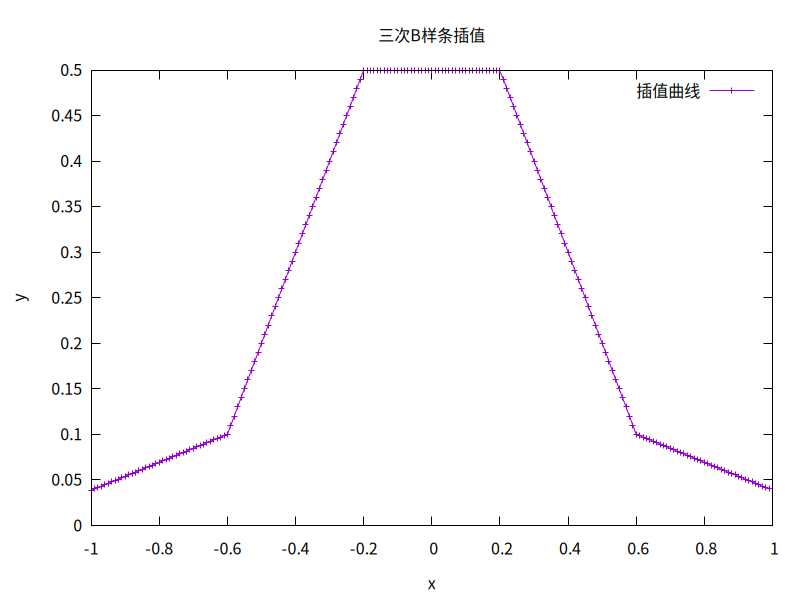
\includegraphics[scale=0.2]{../figure/AL6.png}
    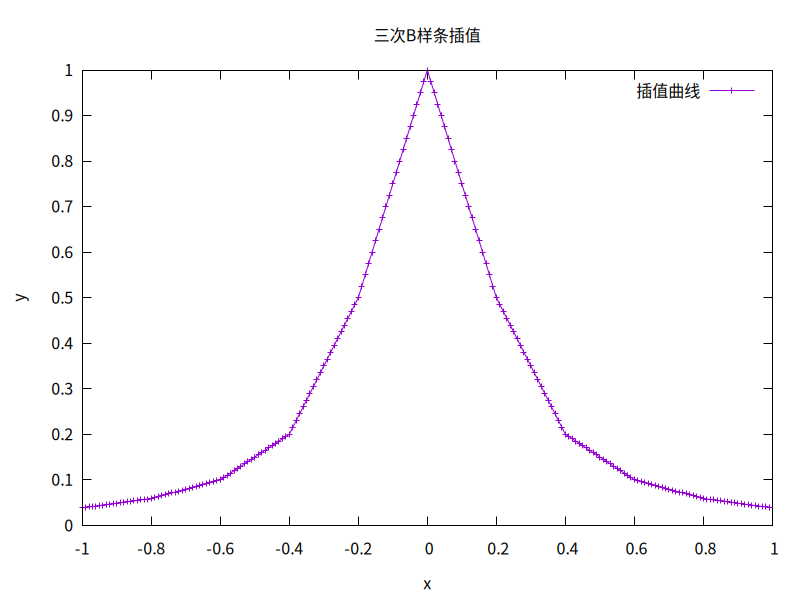
\includegraphics[scale=0.2]{../figure/AL11.png}
    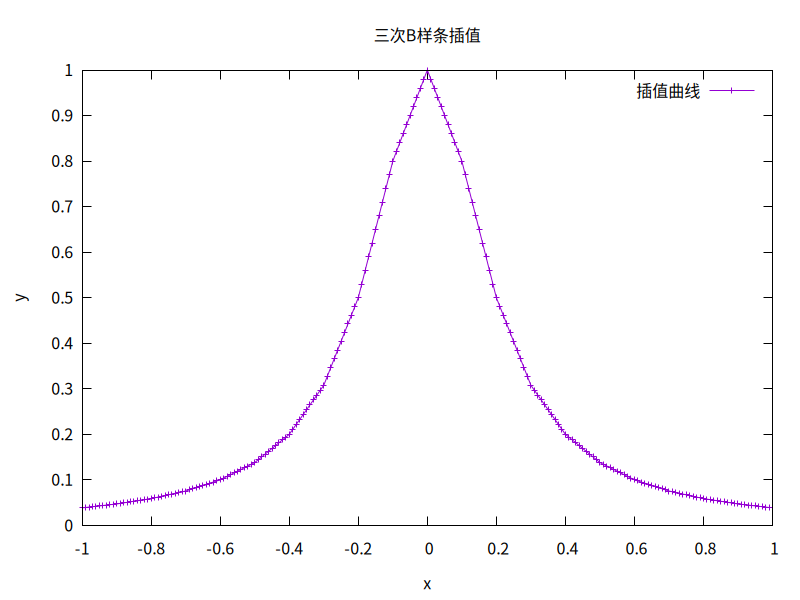
\includegraphics[scale=0.2]{../figure/AL21.png}
    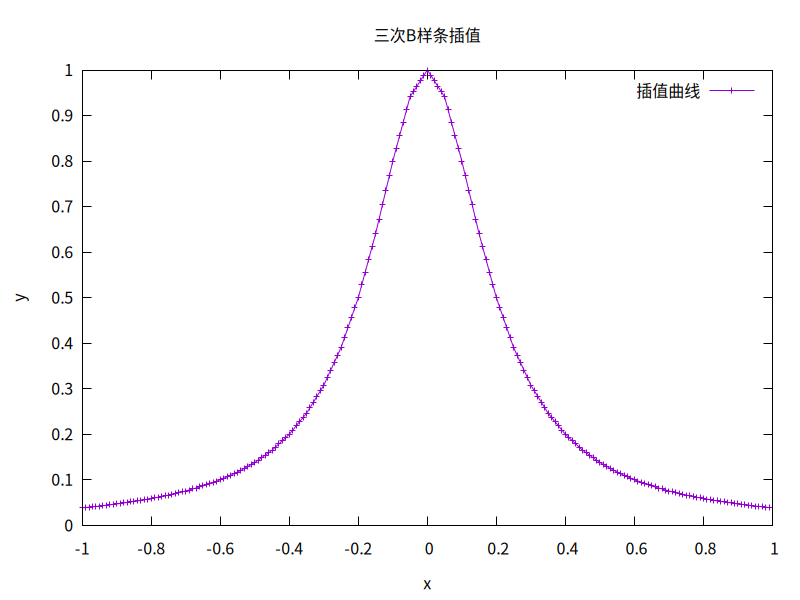
\includegraphics[scale=0.2]{../figure/AL41.png}
    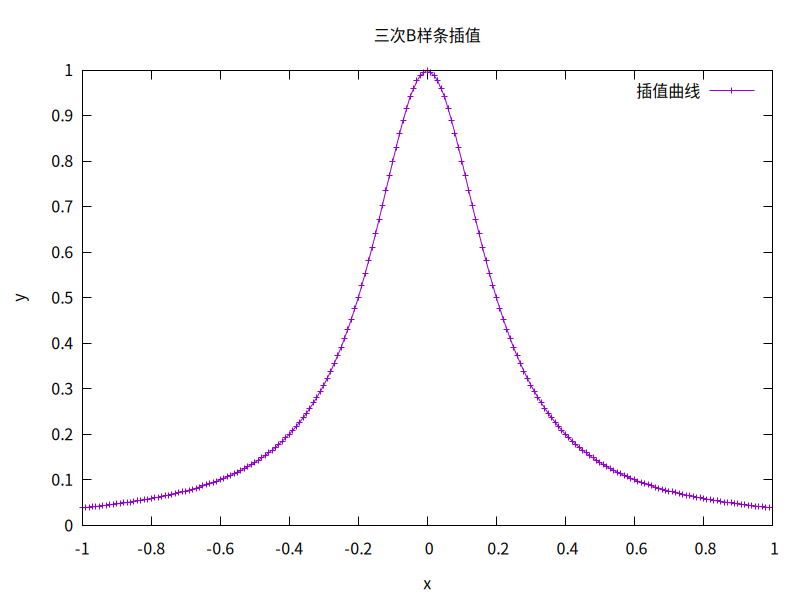
\includegraphics[scale=0.2]{../figure/AL81.png}
    \caption{N=6, N=11, N=21, N=41, N=81}
\end{figure}

\textbf{linear BSpline}
\begin{figure}[H]
    \centering
    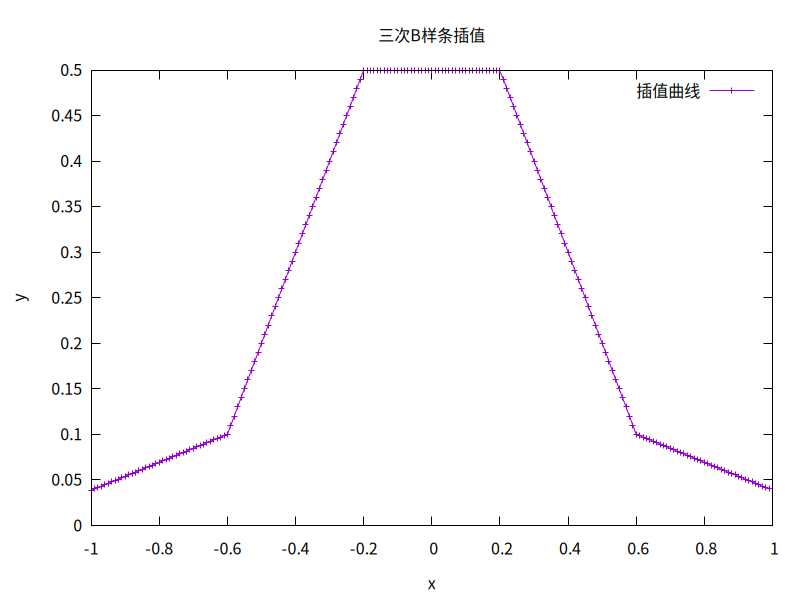
\includegraphics[scale=0.2]{../figure/AL6.png}
    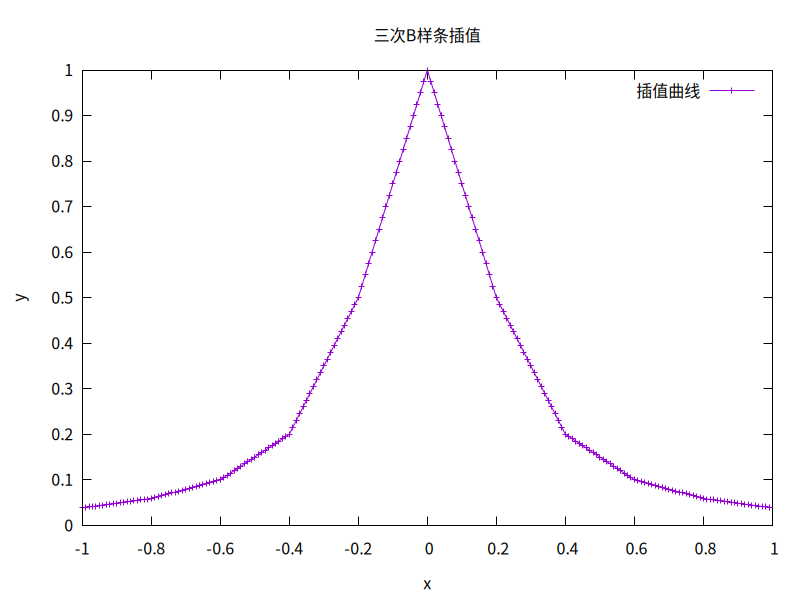
\includegraphics[scale=0.2]{../figure/AL11.png}
    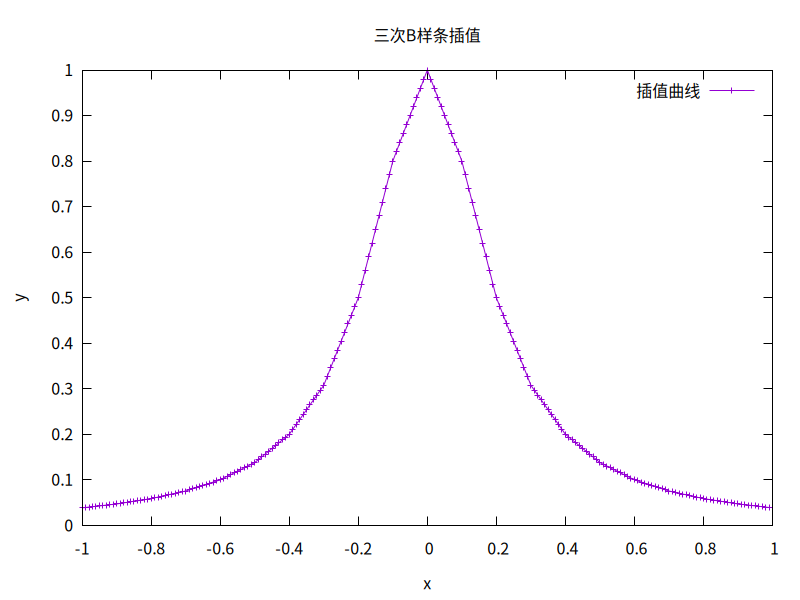
\includegraphics[scale=0.2]{../figure/AL21.png}
    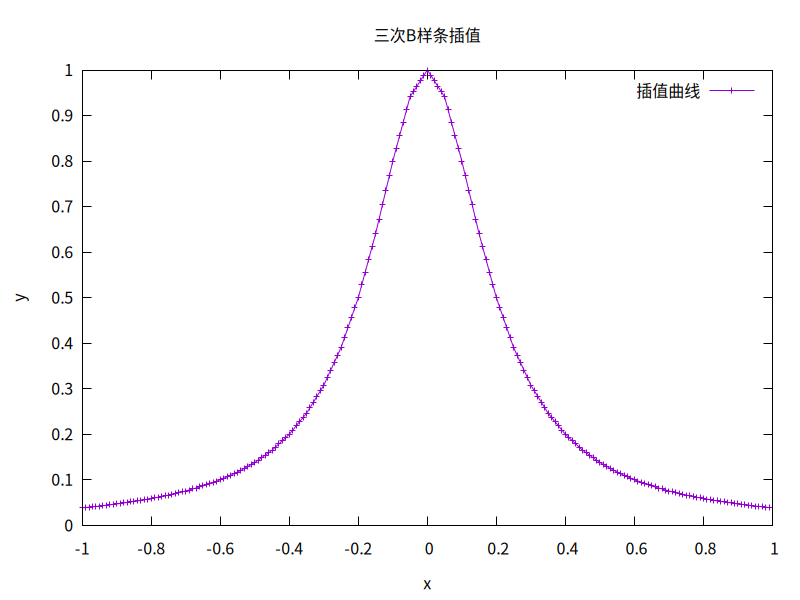
\includegraphics[scale=0.2]{../figure/AL41.png}
    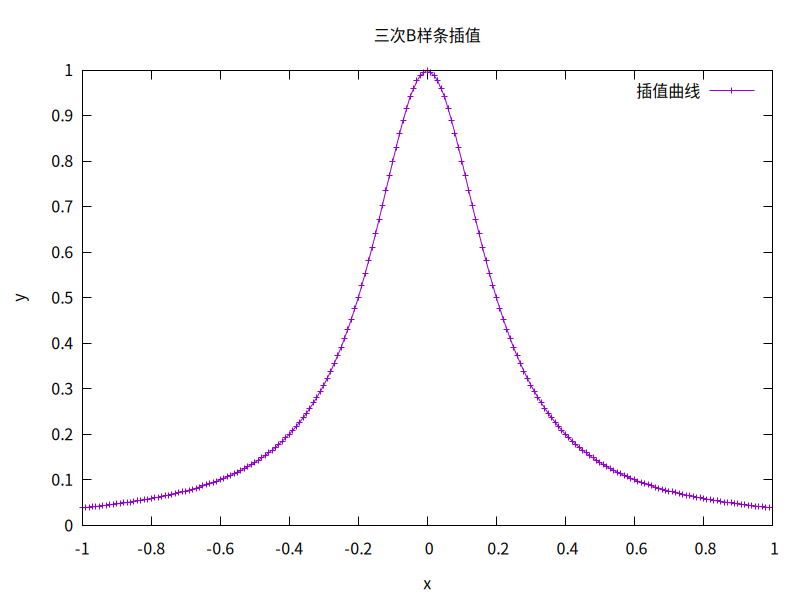
\includegraphics[scale=0.2]{../figure/AL81.png}
    \caption{N=6, N=11, N=21, N=41, N=81}
\end{figure}

\textbf{Natural ppForm Spline}
\begin{lstlisting}
cubic-ppForm_Spline_Error
N = 6 -> Errormax: 0.423856
N = 11 -> Errormax: 0.042903
N = 21 -> Errormax: 0.0136586
N = 41 -> Errormax: 0.00371266
N = 81 -> Errormax: 0.000961739
\end{lstlisting}

\begin{figure}[H]
    \centering
    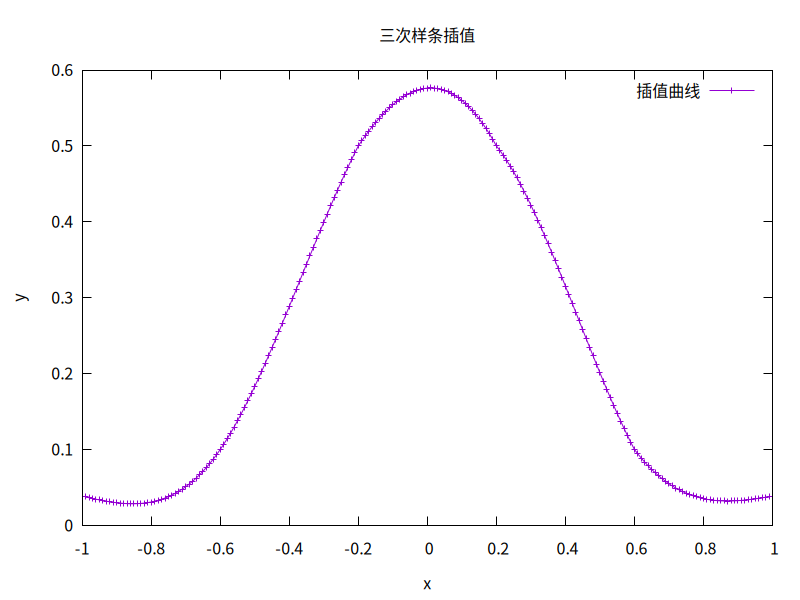
\includegraphics[scale=0.2]{../figure/A6.png}
    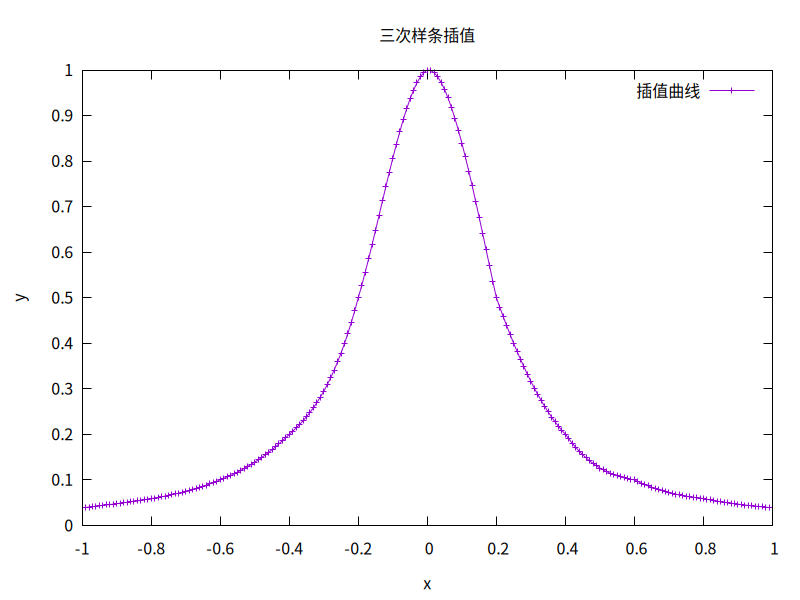
\includegraphics[scale=0.2]{../figure/A11.png}
    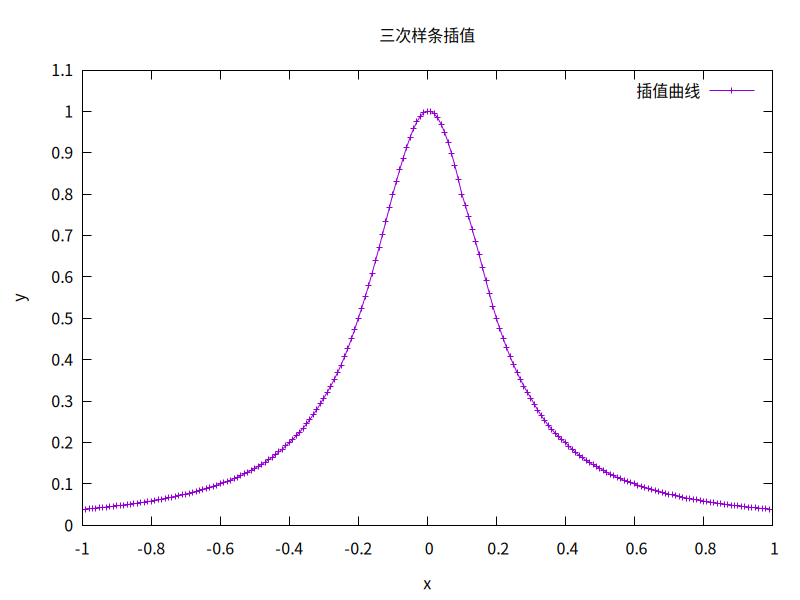
\includegraphics[scale=0.2]{../figure/A21.png}
    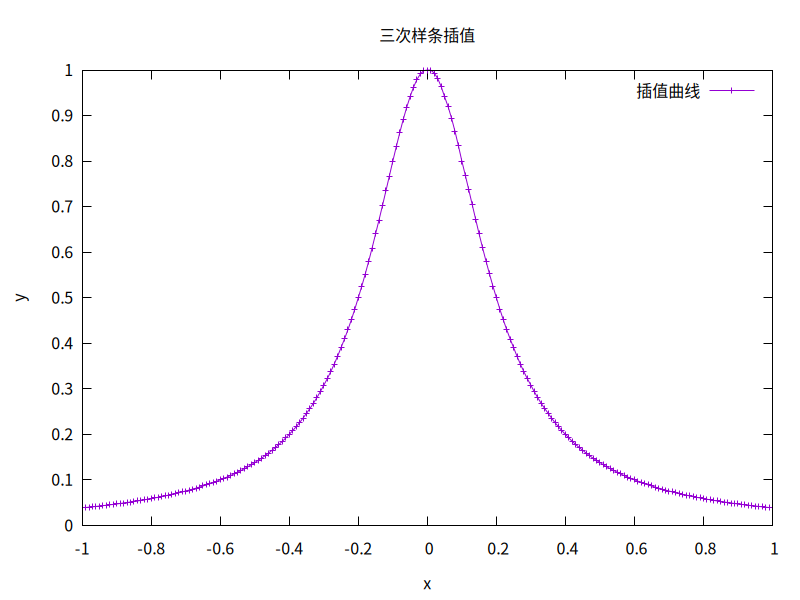
\includegraphics[scale=0.2]{../figure/A41.png}
    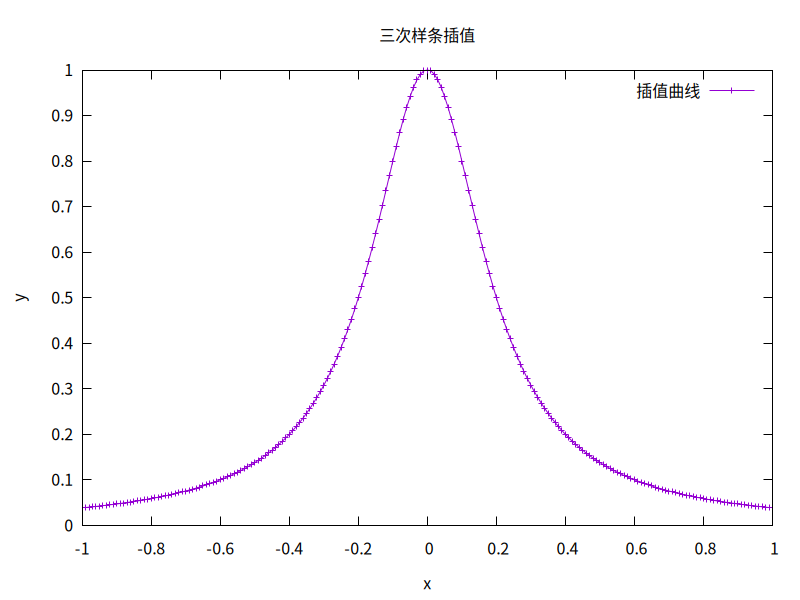
\includegraphics[scale=0.2]{../figure/A81.png}
    \caption{N=6, N=11, N=21, N=41, N=81}
\end{figure}

\textbf{Complete ppForm Spline}
\begin{figure}[H]
    \centering
    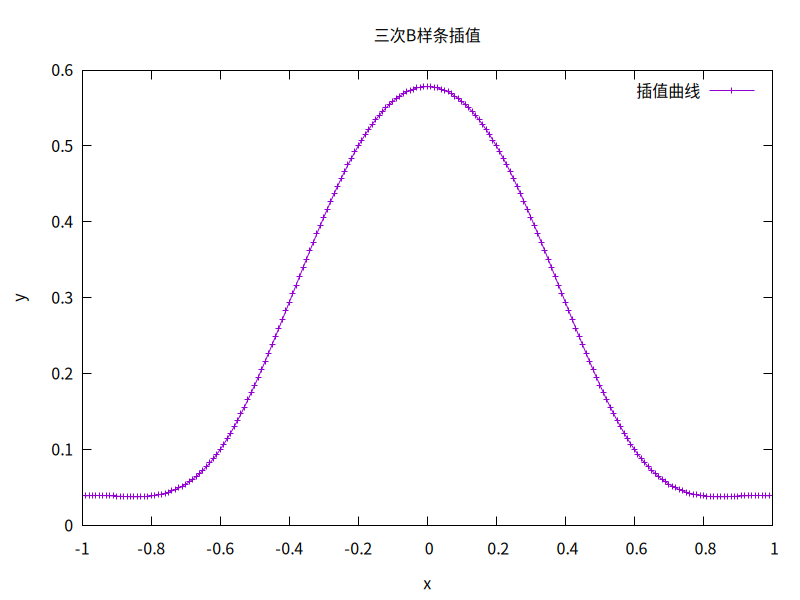
\includegraphics[scale=0.2]{../figure/APC6.png}
    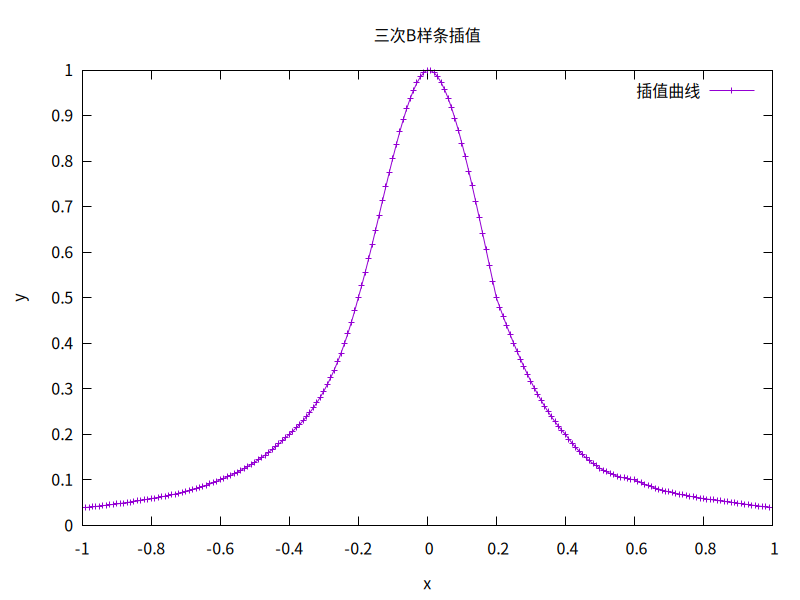
\includegraphics[scale=0.2]{../figure/APC11.png}
    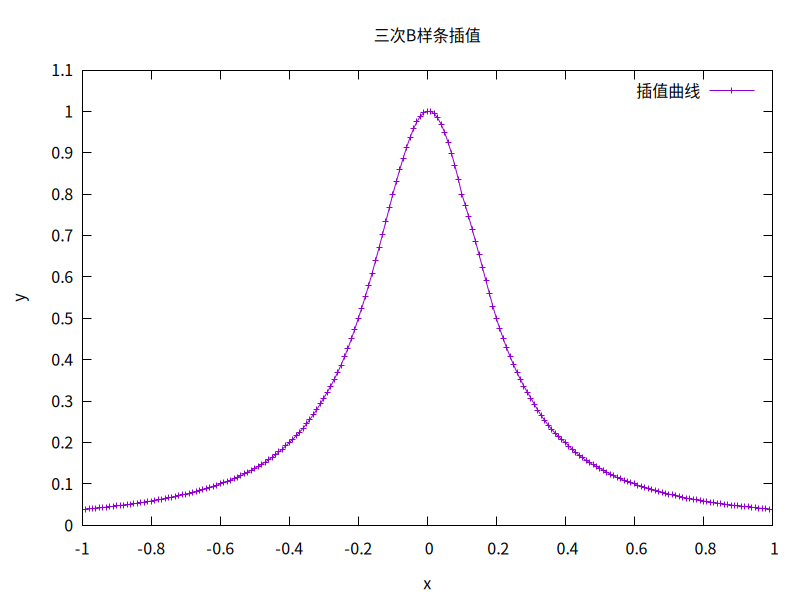
\includegraphics[scale=0.2]{../figure/APC21.png}
    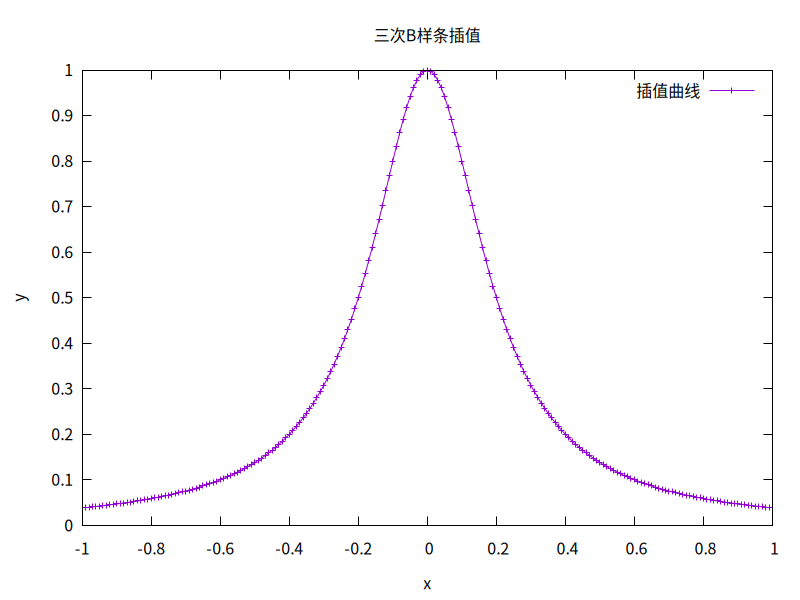
\includegraphics[scale=0.2]{../figure/APC41.png}
    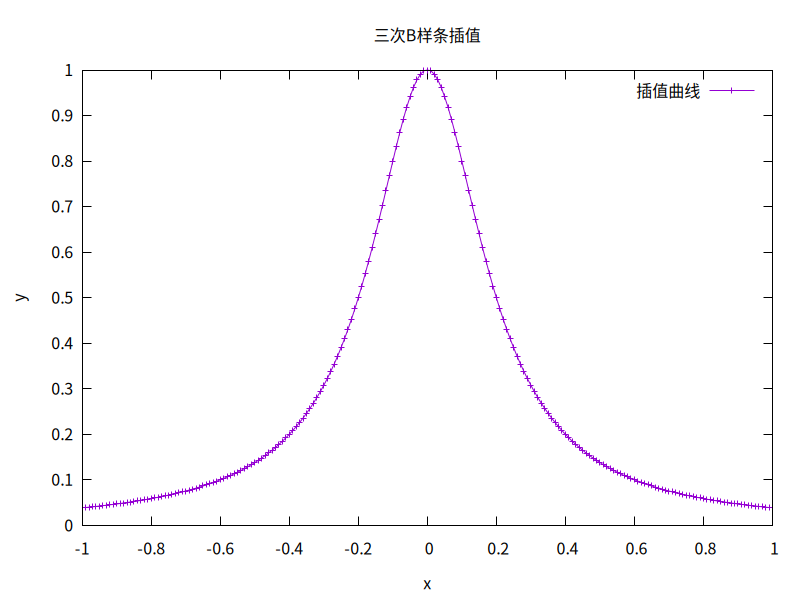
\includegraphics[scale=0.2]{../figure/APC81.png}
    \caption{N=6, N=11, N=21, N=41, N=81}
\end{figure}

\textbf{Natural BSpline}
\begin{figure}[H]
    \centering
    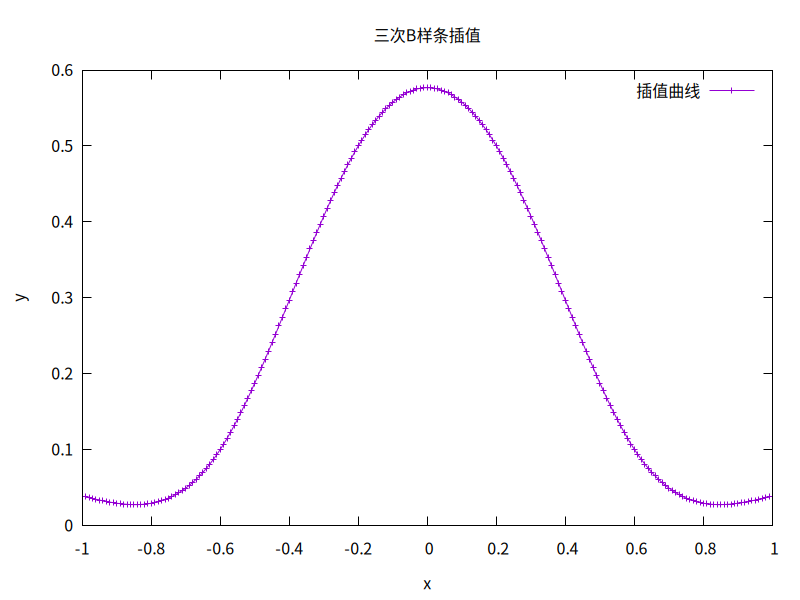
\includegraphics[scale=0.2]{../figure/ABN6.png}
    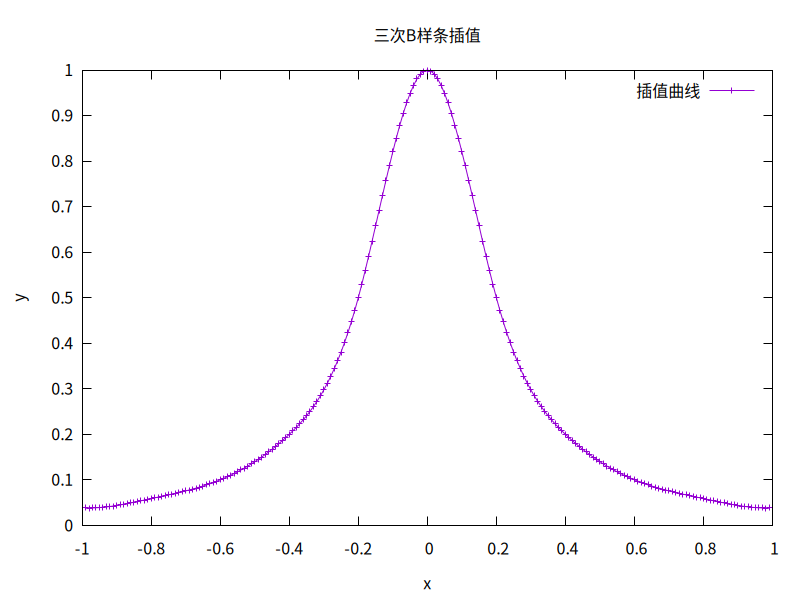
\includegraphics[scale=0.2]{../figure/ABN11.png}
    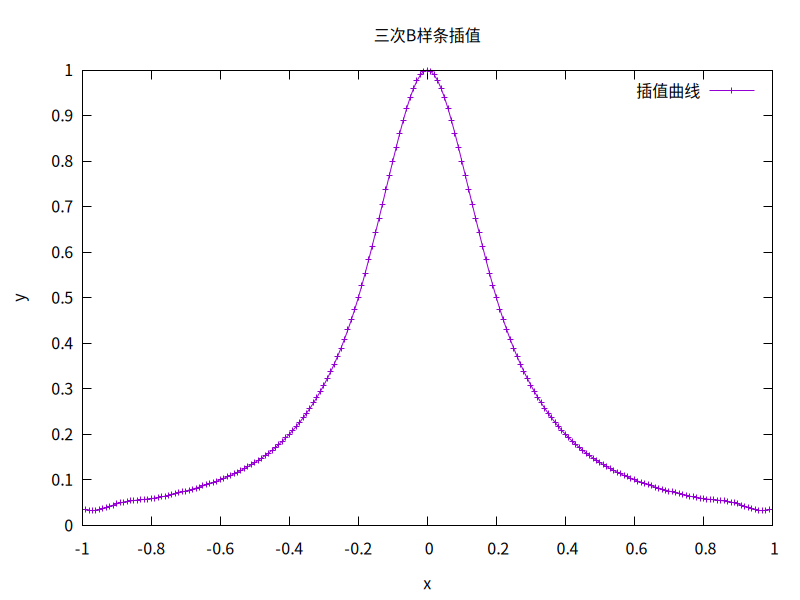
\includegraphics[scale=0.2]{../figure/ABN21.png}
    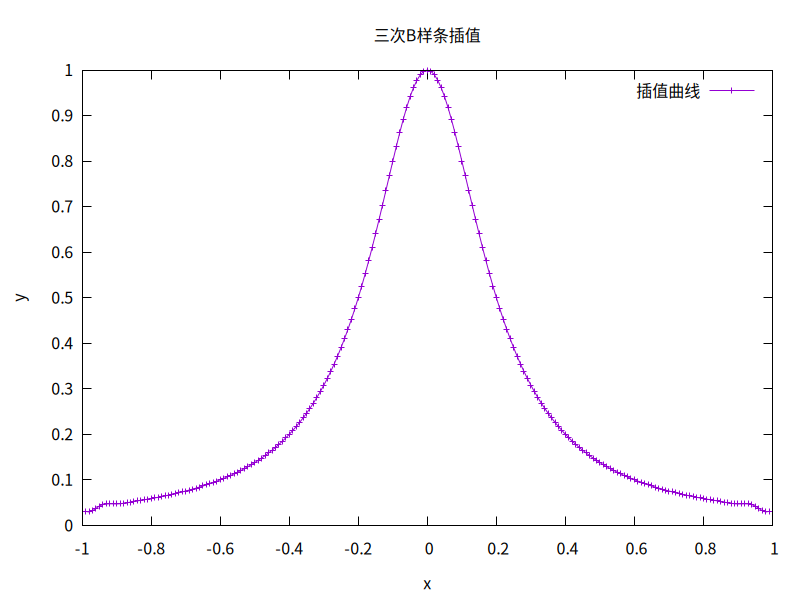
\includegraphics[scale=0.2]{../figure/ABN41.png}
    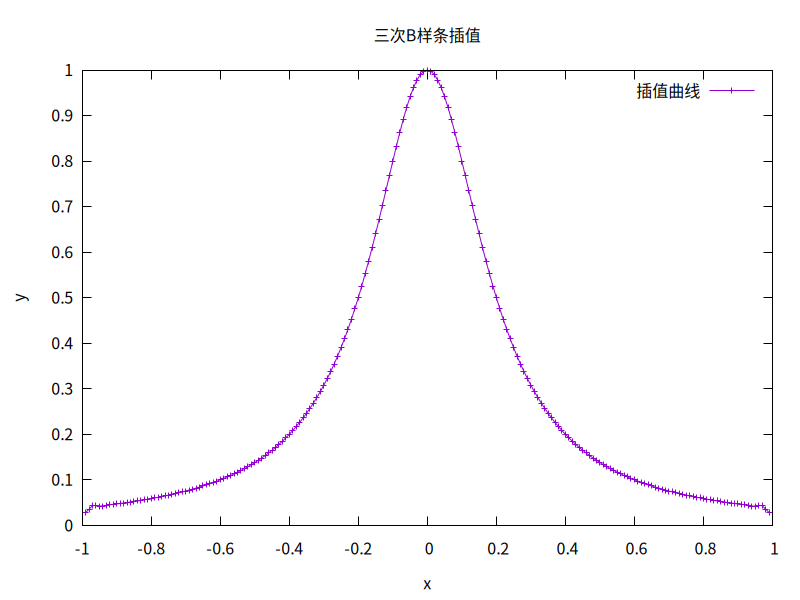
\includegraphics[scale=0.2]{../figure/ABN81.png}
    \caption{N=6, N=11, N=21, N=41, N=81}
\end{figure}

\textbf{Complete BSpline}
\begin{figure}[H]
    \centering
    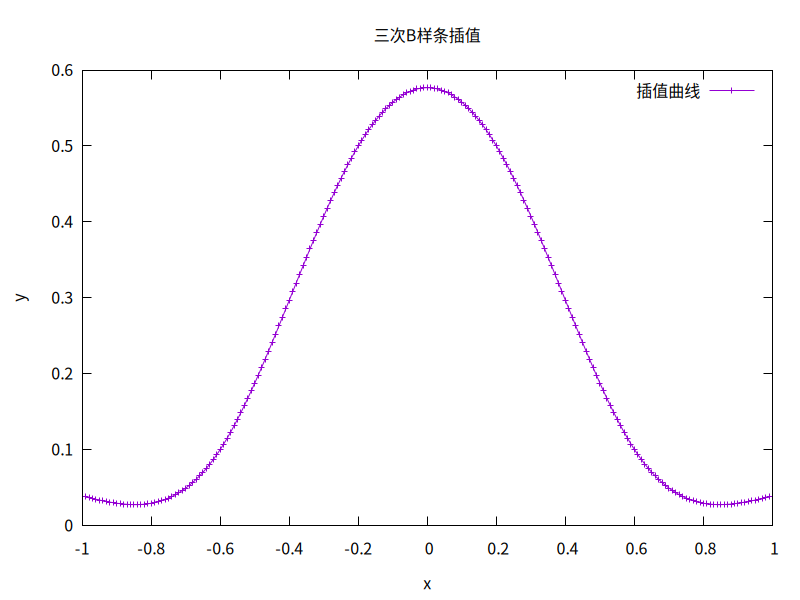
\includegraphics[scale=0.2]{../figure/ABC6.png}
    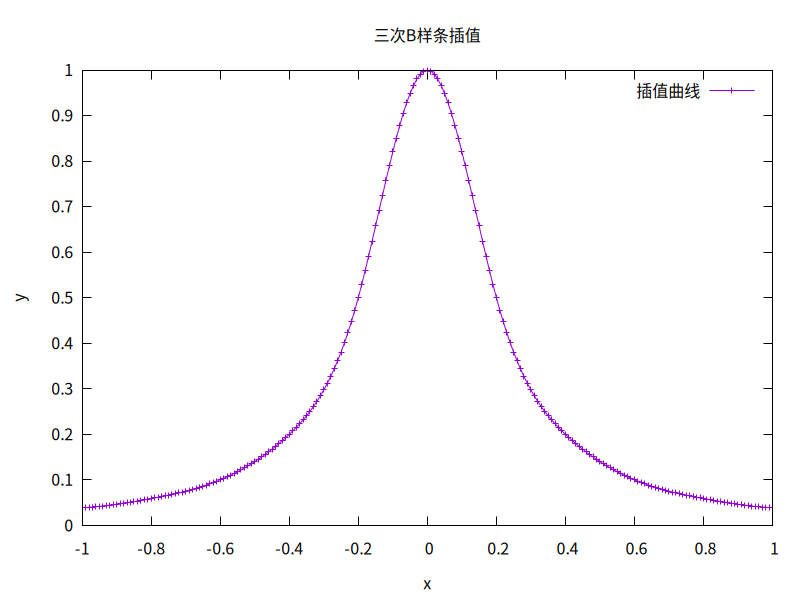
\includegraphics[scale=0.2]{../figure/ABC11.png}
    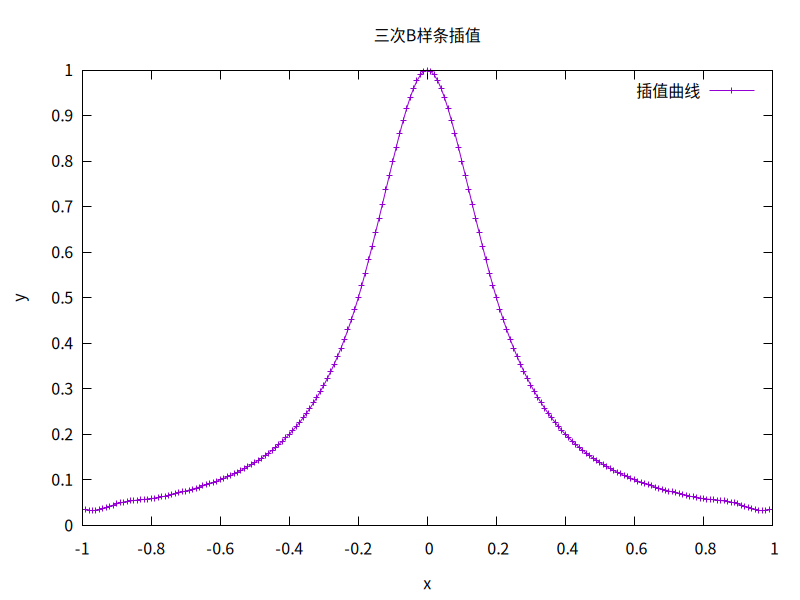
\includegraphics[scale=0.2]{../figure/ABC21.png}
    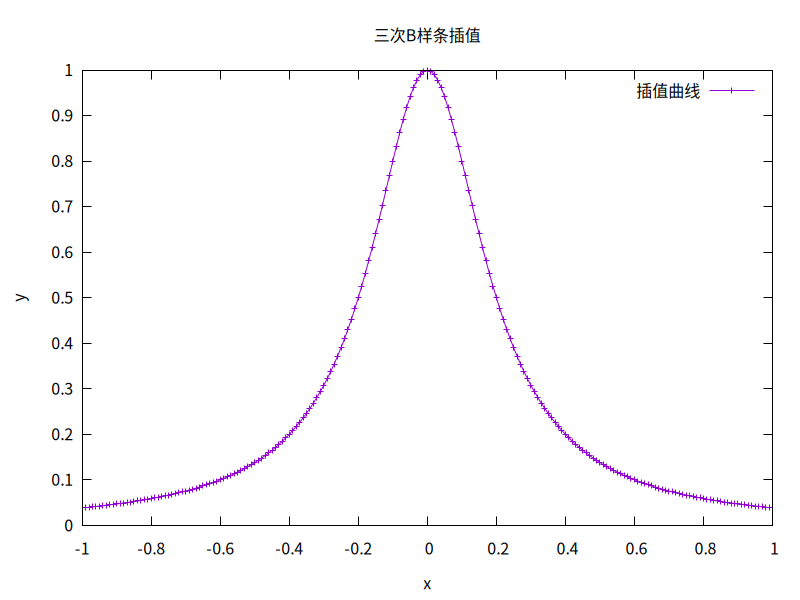
\includegraphics[scale=0.2]{../figure/ABC41.png}
    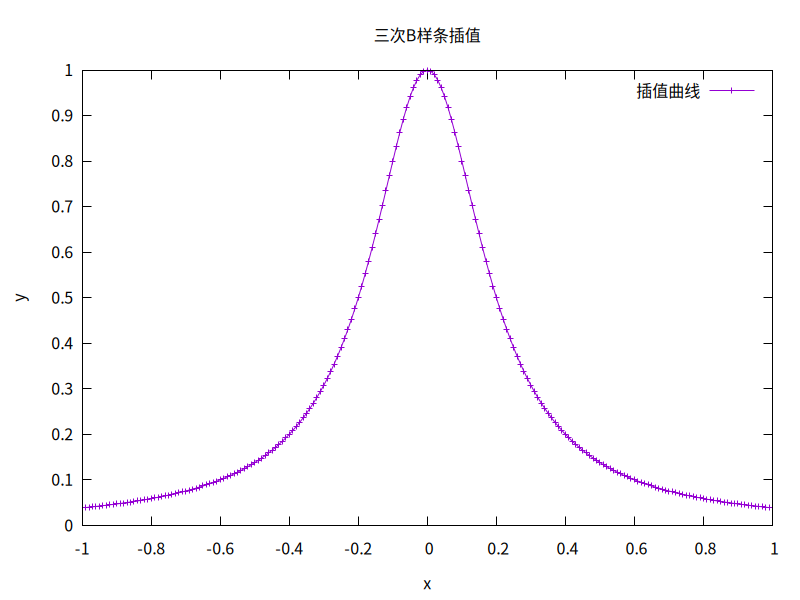
\includegraphics[scale=0.2]{../figure/ABC81.png}
    \caption{N=6, N=11, N=21, N=41, N=81}
\end{figure}
验证发现ppform和BSpline在相同边界条件下获得的插值曲线基本相同。



\subsection*{C}
拟合结果如图所示：
\begin{figure}[H]
    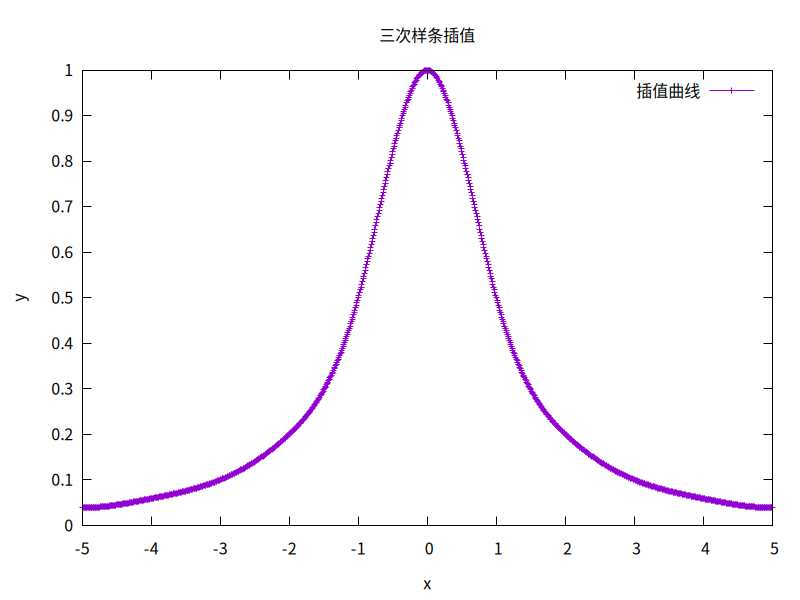
\includegraphics[scale=0.3]{../figure/B357.png}
    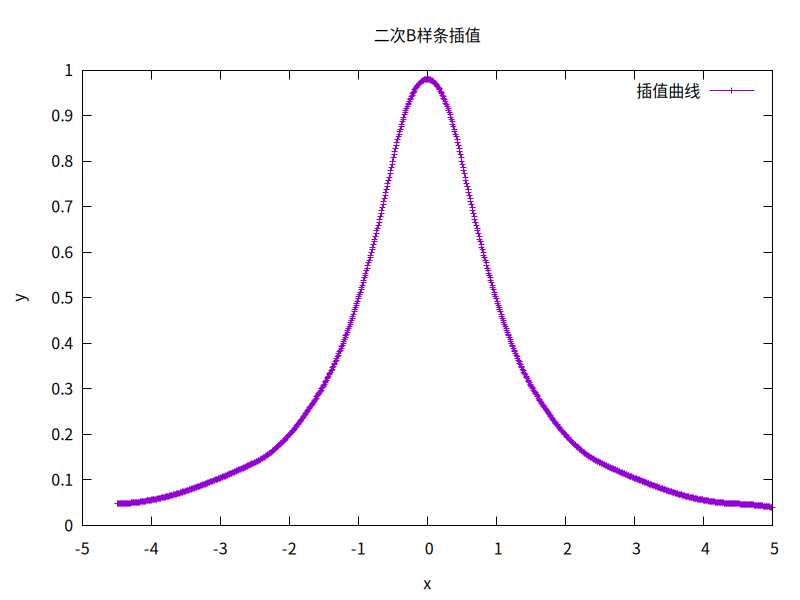
\includegraphics[scale=0.3]{../figure/B358.png}
    \caption{$\mathbb{S} _{3}^{2}$, $\mathbb{S} _{2}^{1}$}
\end{figure}

分别按题意要求画出拟合曲线（左右）。

\subsection*{D}
\subsubsection*{$\mathbb{S} _{3}^{2}$}
\begin{lstlisting}
x = -3.5 -> Error: 0.000460179
x = -3 -> Error: 5.55112e-17
x = -0.5 -> Error: 0.0205259
x = 0 -> Error: 0
x = 0.5 -> Error: 0.0205259
x = 3 -> Error: 5.55112e-17
x = 3.5 -> Error: 0.000460179
\end{lstlisting}

\subsubsection*{$\mathbb{S} _{2}^{1}$}
\begin{lstlisting}
x = -3.5 -> Error: 4.16334e-17
x = -3 -> Error: 0.00397321
x = -0.5 -> Error: 0
x = 0 -> Error: Error: 0.0203838
x = 0.5 -> Error: 0
x = 3 -> Error: 0.00397321
x = 3.5 -> Error: 4.16334e-17
\end{lstlisting}

有些点的误差接近机器精度的原因是那些点就是用于拟合的插值点，因此误差为0或极小。

\subsection*{E}
\subsection*{实现}
为了计算cumulaive chordal length，我们需要计算每个节点的长度，并将其累加。因为一些函数的$r(s)$表达式复杂或无法求得，
我的做法是先手算出$s(t) = \int_{0}^{t} \left\lVert r^{'}(t)\right\rVert _{2}  \,dx $的表达式，
将这个表达式写成一个Function类fs（Function类中定义了二分法），在fs中重载运算符+ ，用于应用二分法求出每小段弧长对应的t值。

\begin{lstlisting}
class Function{
public:
    virtual double operator()(double x) const = 0;
    virtual double derivative(double x) const;
    virtual ~Function(){}
    double bisection_method(double a, double b, double tolerance = 1e-6, int max_iterations = 100);
};

class f2s:public Function{
public:
    double operator()(double x);
    Function* operator+(double value) {
        class AddedFunction : public Function{
        public:
            const f2s& baseFunction;
            double addtionalValue;
            AddedFunction(const f2s& f, double v): baseFunction(f), addtionalValue(v);
            double operator()(double x) const override;
        return new AddedFunction(*this, value);
        }
    }
} 
\end{lstlisting}
Function类的具体代码在Function.h中, f2s在problem.cpp中。

\subsubsection*{心形线}
\textbf{原图}
\begin{figure}[H]
    \centering
    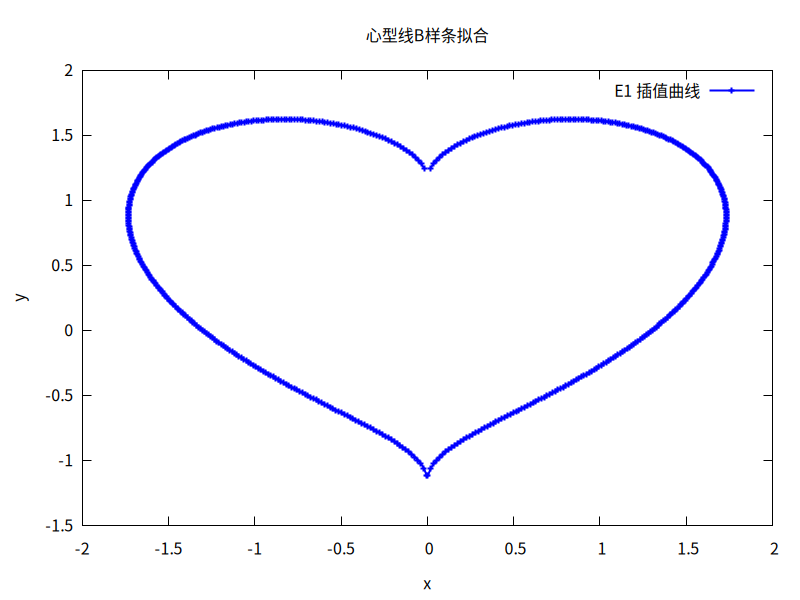
\includegraphics[scale=0.25]{../figure/E_real.png}
\end{figure}

本题与前面的样条拟合与所不同。该题要求完成绘制的是一个闭合曲线，但是注意到心形线关于y轴对称，
故只需拟合图片的左半部分，完成后对称得到右半部分。
将函数写成参数形式：
$$
\left\{
\begin{aligned}
    x(t) &= \sqrt{3} \sin(t) \\
    y(t) &= \frac{2}{3}\left(\sqrt{3} \cos(t) + \sqrt{\sqrt{3} \sin(t)}\right)
\end{aligned}
\right.
$$


以下是使用等距节点拟合心形线的结果：

\textbf{Natural}
\begin{figure}[H]
    \centering
    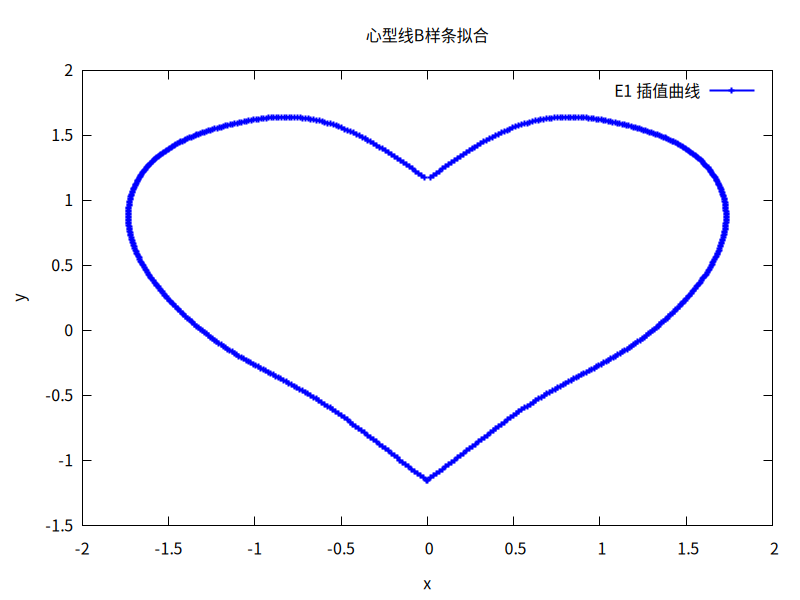
\includegraphics[scale=0.15]{../figure/EN10.png}
    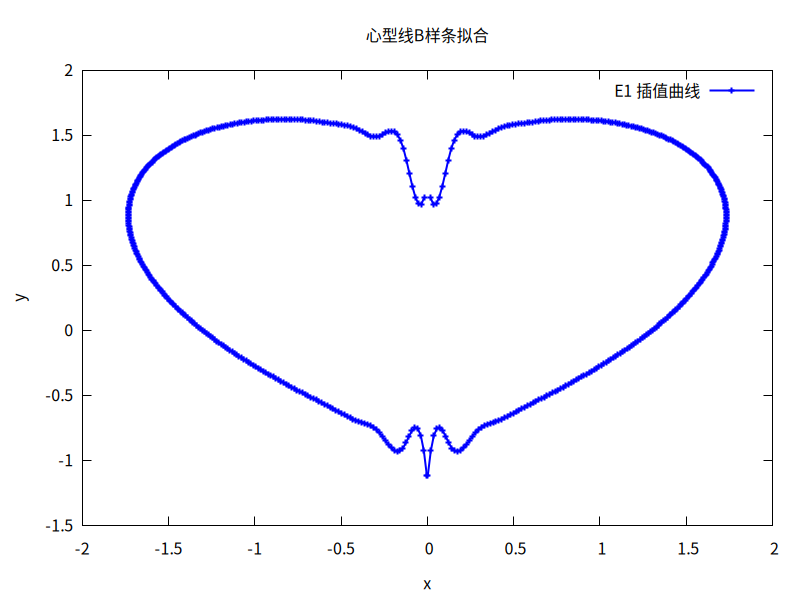
\includegraphics[scale=0.15]{../figure/EN40.png}
    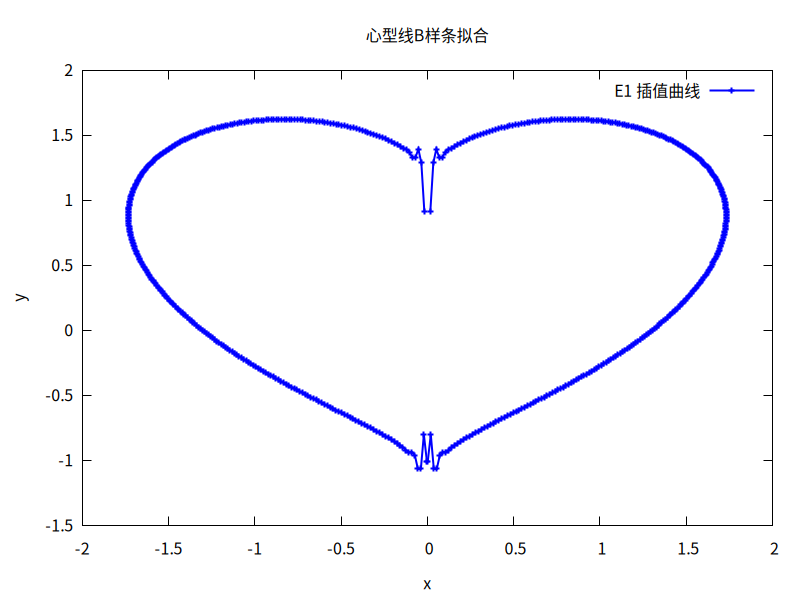
\includegraphics[scale=0.15]{../figure/EN160.png}
    \caption{N=10, N=40, N=160}
\end{figure}
\textbf{Complete}
\begin{figure}[H]
    \centering
    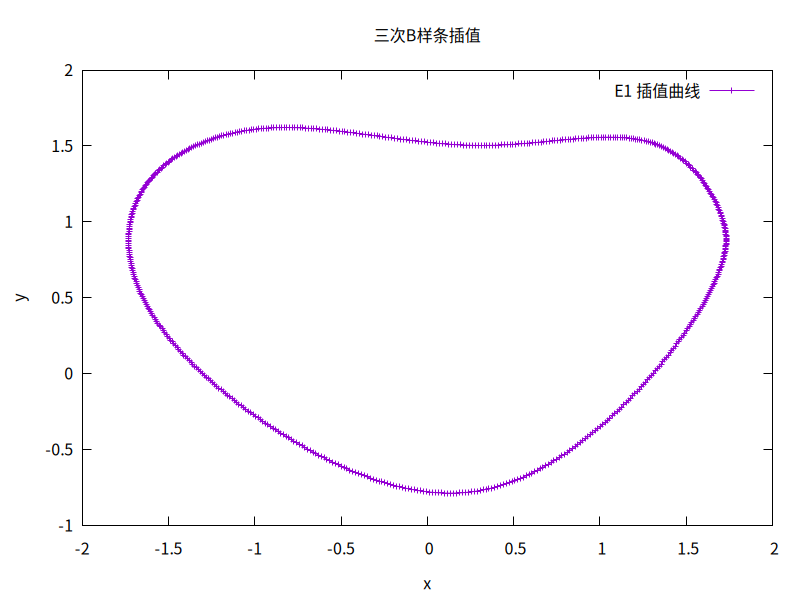
\includegraphics[scale=0.15]{../figure/EC10.png}
    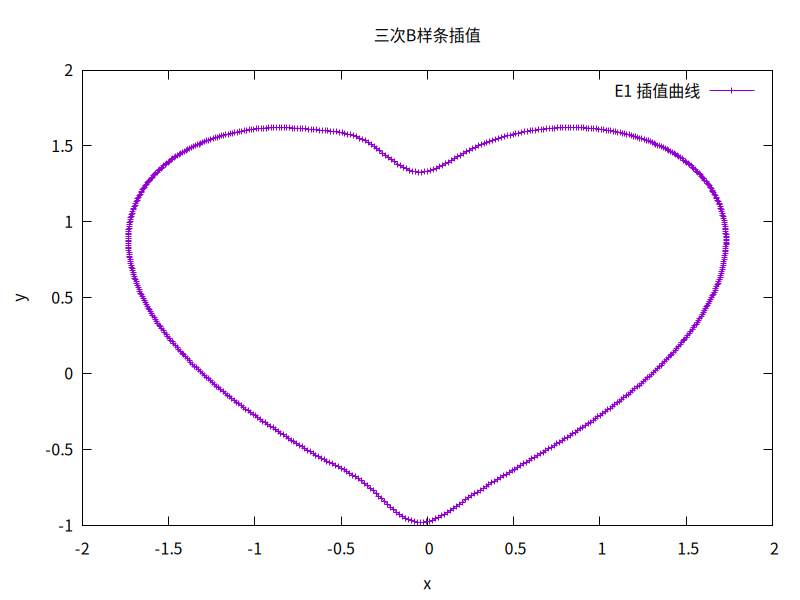
\includegraphics[scale=0.15]{../figure/EC40.png}
    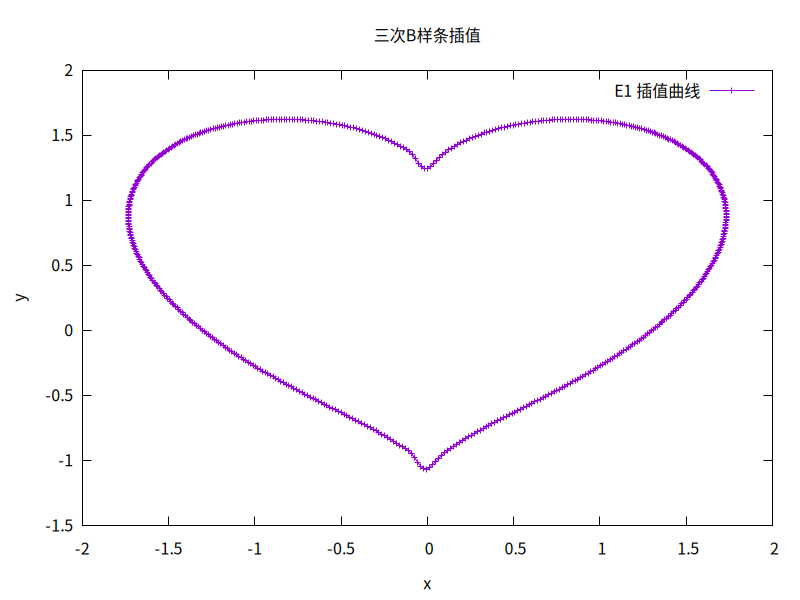
\includegraphics[scale=0.15]{../figure/EC160.png}
    \caption{N=10, N=40, N=160}
\end{figure}
\textbf{Periodic}
\begin{figure}[H]
    \centering
    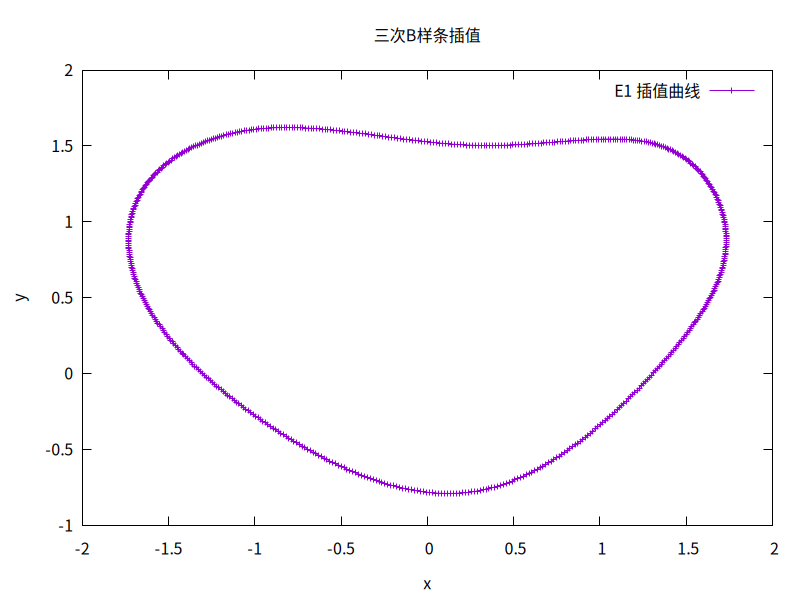
\includegraphics[scale=0.15]{../figure/EP10.png}
    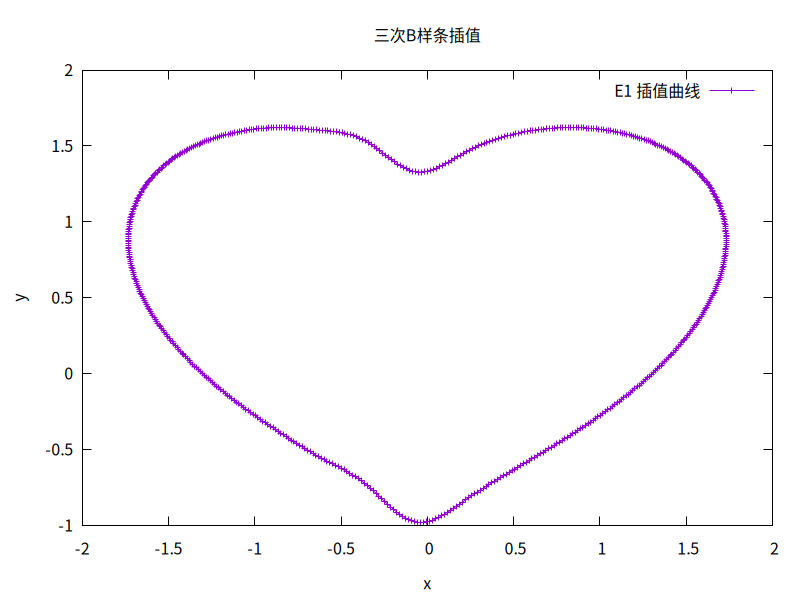
\includegraphics[scale=0.15]{../figure/EP40.png}
    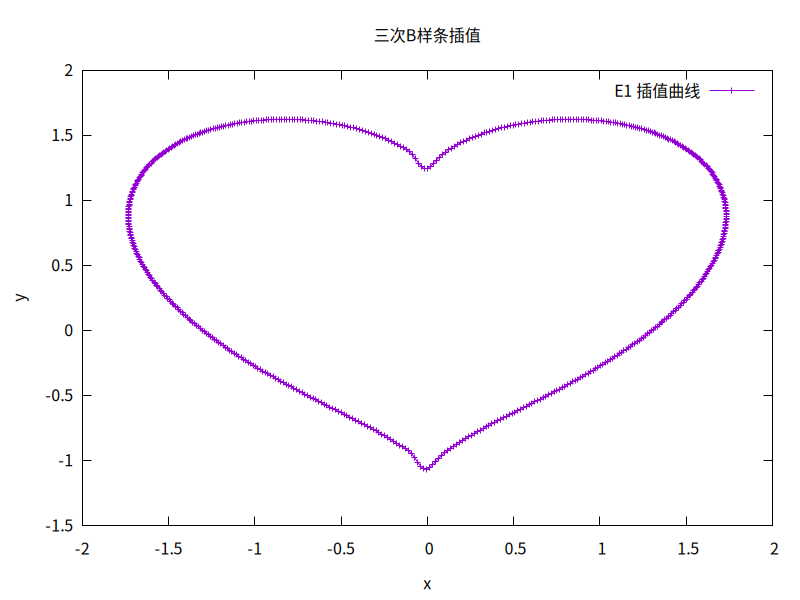
\includegraphics[scale=0.15]{../figure/EP160.png}
    \caption{N=10, N=40, N=160}
\end{figure}

发现Natural条件下，由于在边界点$0$,$ \pi$处函数不可导，导致在边界处插值函数值不准确。
解决办法是应用cumulative chordal length方法在边界处使用更多节点，加强b样条在边界处的准确性。

结果如下：
\textbf{Natural}
\begin{figure}[H]
    \centering
    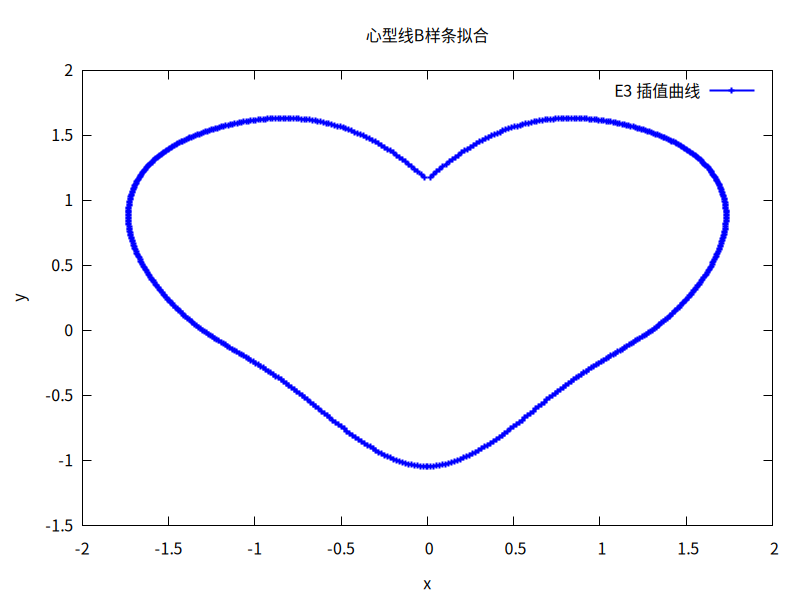
\includegraphics[scale=0.15]{../figure/ENC10.png}
    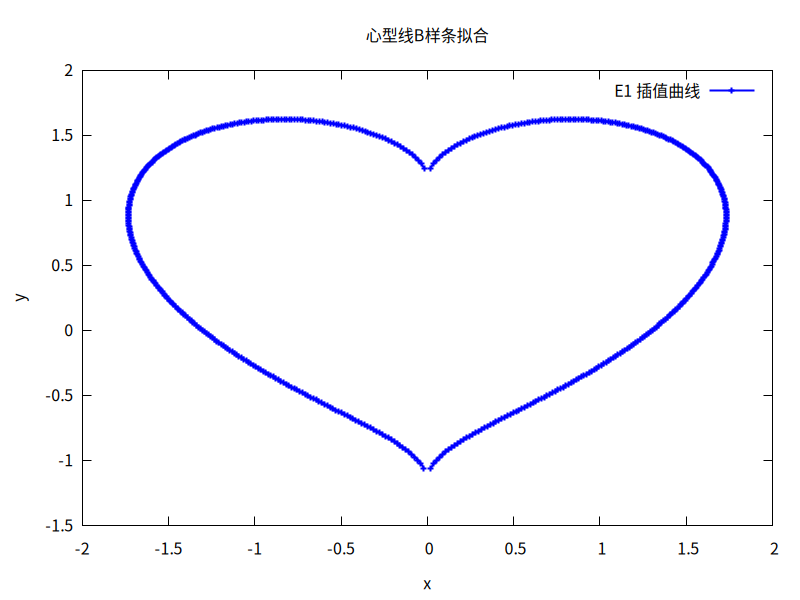
\includegraphics[scale=0.15]{../figure/ENC40.png}
    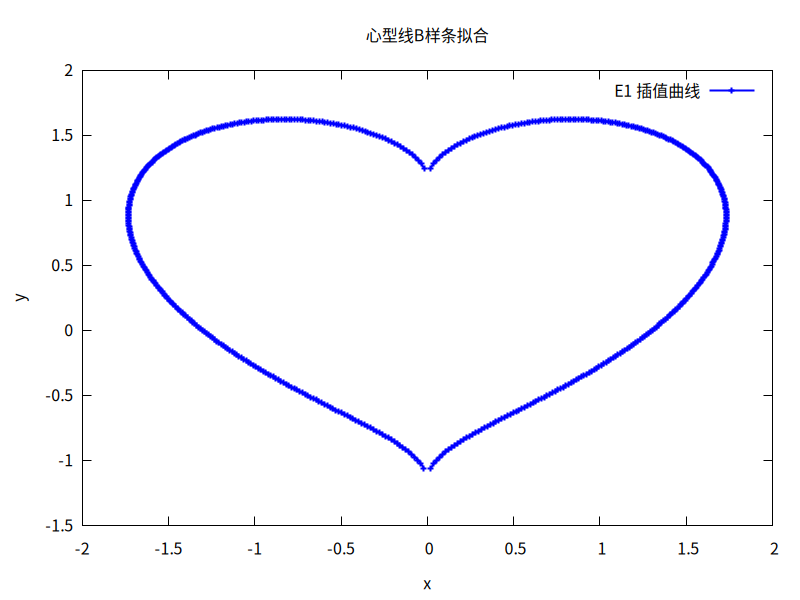
\includegraphics[scale=0.15]{../figure/ENC160.png}
    \caption{N=10, N=40, N=160}
\end{figure}
\textbf{Complete}
\begin{figure}[H]
    \centering
    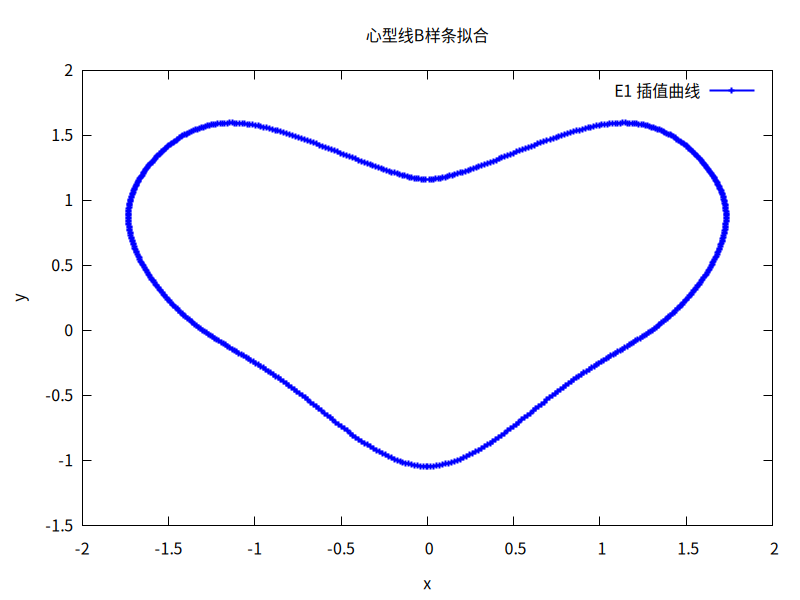
\includegraphics[scale=0.15]{../figure/ECC10.png}
    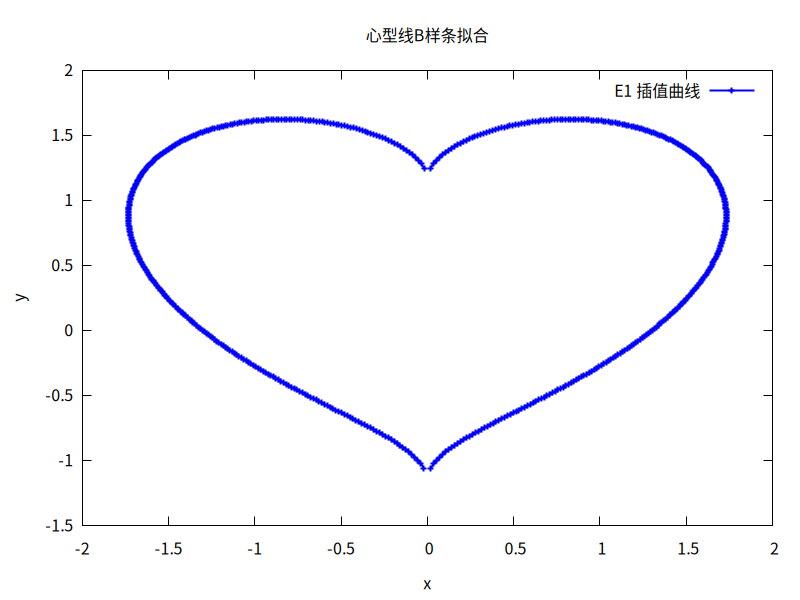
\includegraphics[scale=0.15]{../figure/ECC40.png}
    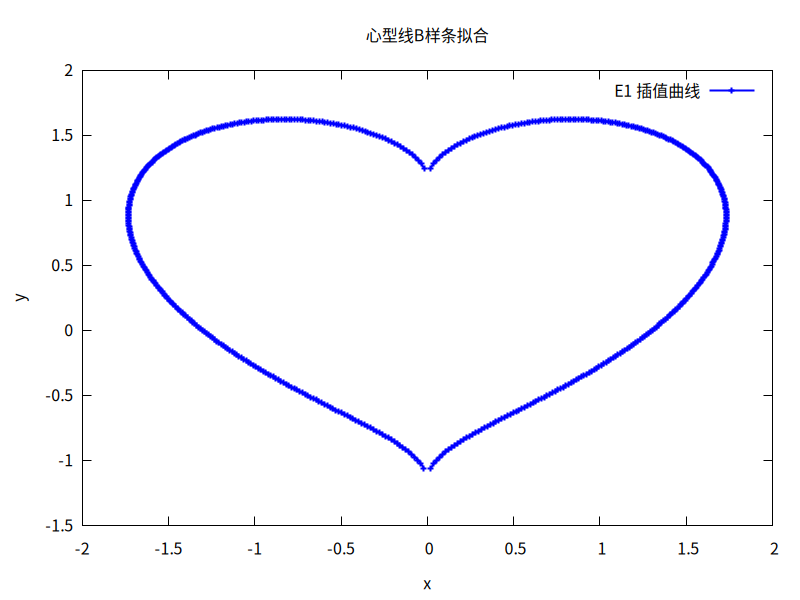
\includegraphics[scale=0.15]{../figure/ECC160.png}
    \caption{N=10, N=40, N=160}
\end{figure}
\textbf{Periodic}
\begin{figure}[H]
    \centering
    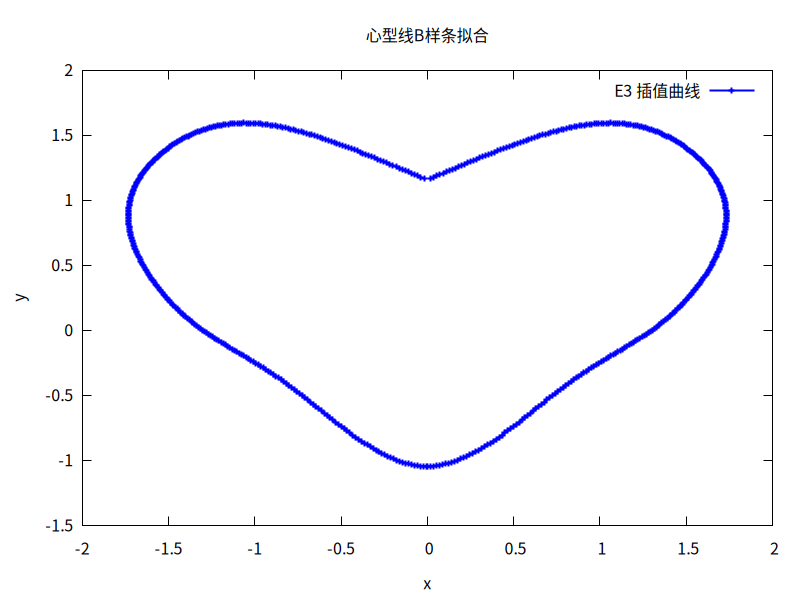
\includegraphics[scale=0.15]{../figure/EPC10.png}
    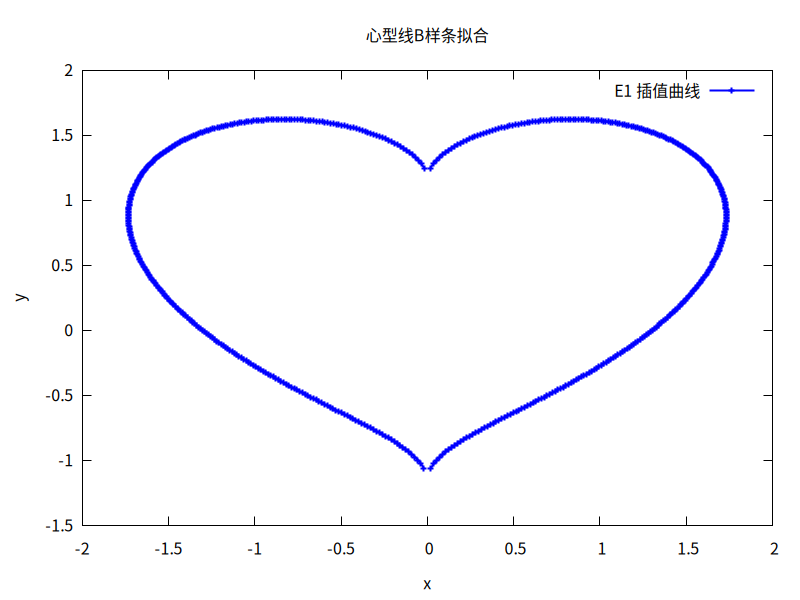
\includegraphics[scale=0.15]{../figure/EPC40.png}
    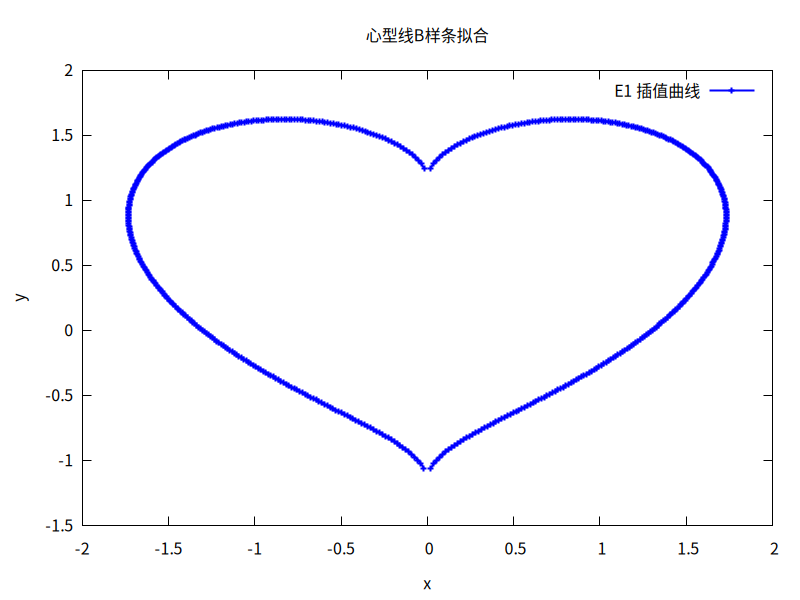
\includegraphics[scale=0.15]{../figure/EPC160.png}
    \caption{N=10, N=40, N=160}
\end{figure}

% \newpage
\subsection*{螺线}
\textbf{原图}
\begin{figure}[H]
    \centering
    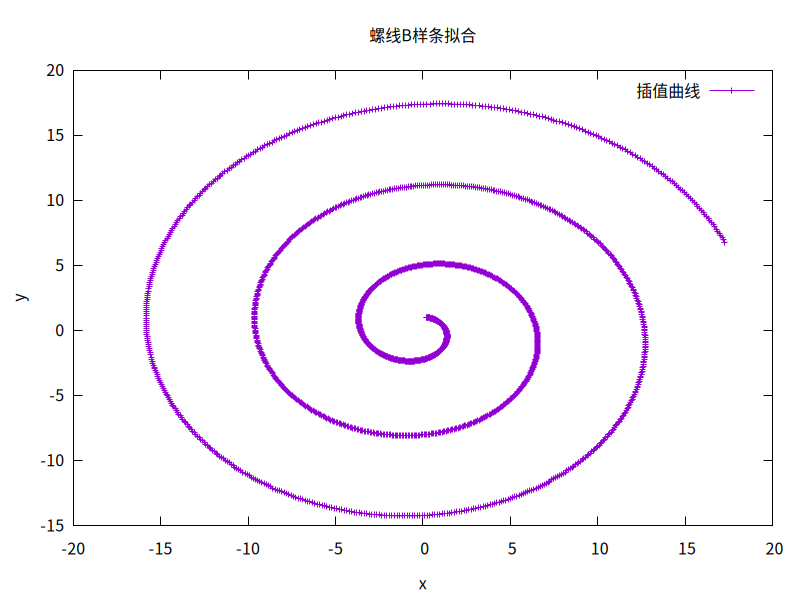
\includegraphics[scale=0.25]{../figure/F_real.png}
\end{figure}
本题给出的函数是光滑的，因此直接拟合即可。

等距节点的拟合结果如下：
\textbf{Natural}
\begin{figure}[H]
    \centering
    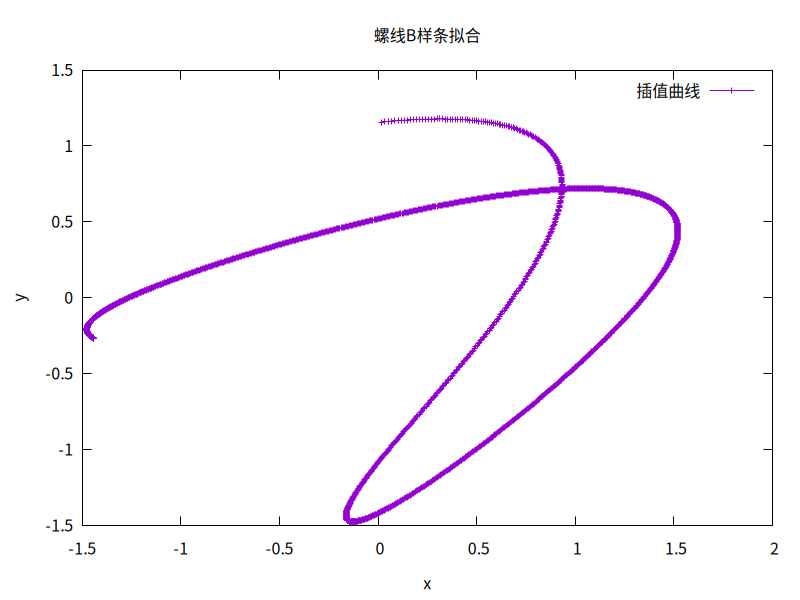
\includegraphics[scale=0.15]{../figure/FN10.png}
    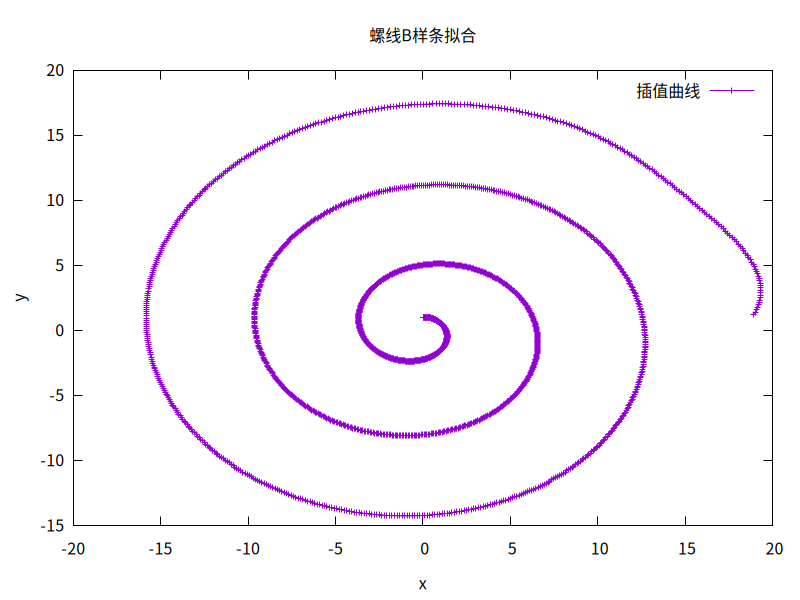
\includegraphics[scale=0.15]{../figure/FN40.png}
    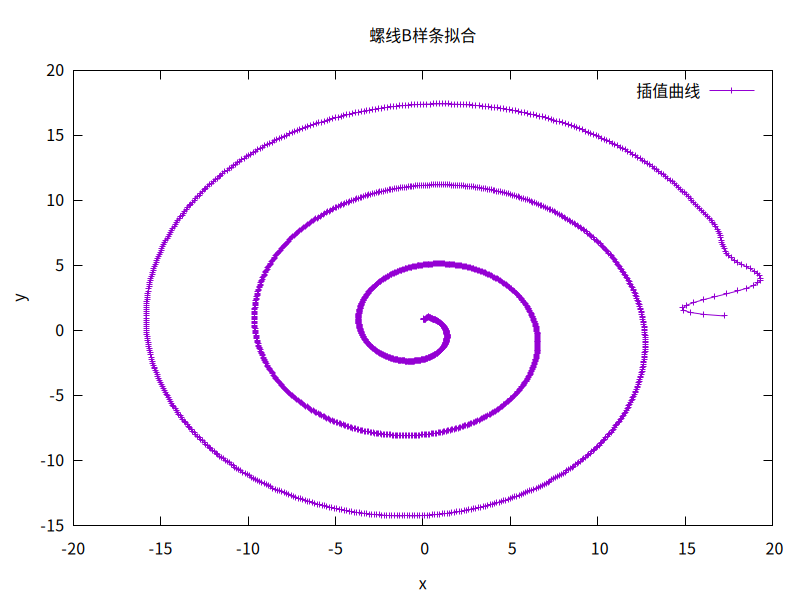
\includegraphics[scale=0.15]{../figure/FN160.png}
    \caption{N=10, N=40, N=160}
\end{figure}
\textbf{Complete}
\begin{figure}[H]
    \centering
    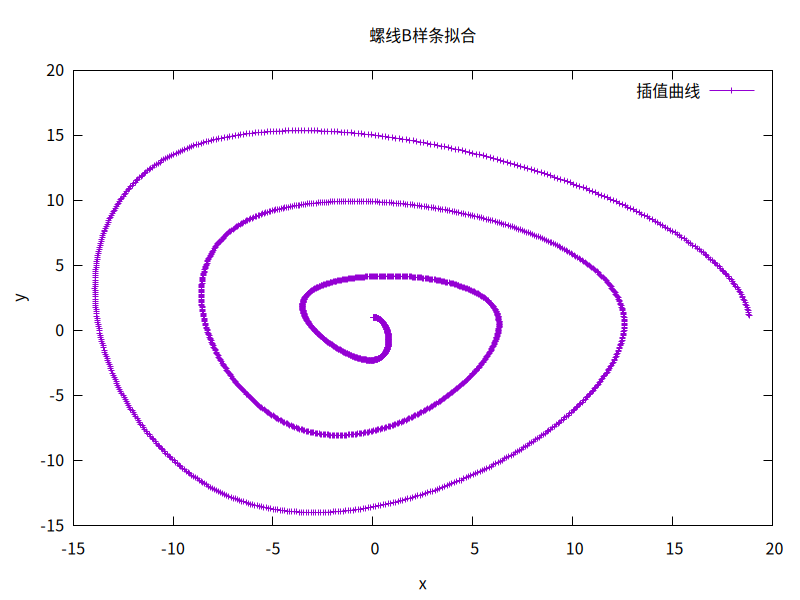
\includegraphics[scale=0.15]{../figure/FC10.png}
    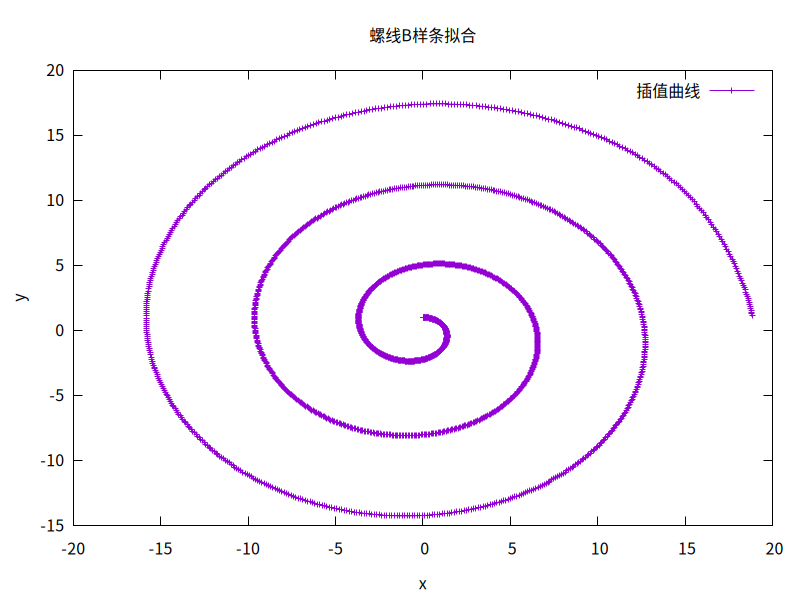
\includegraphics[scale=0.15]{../figure/FC40.png}
    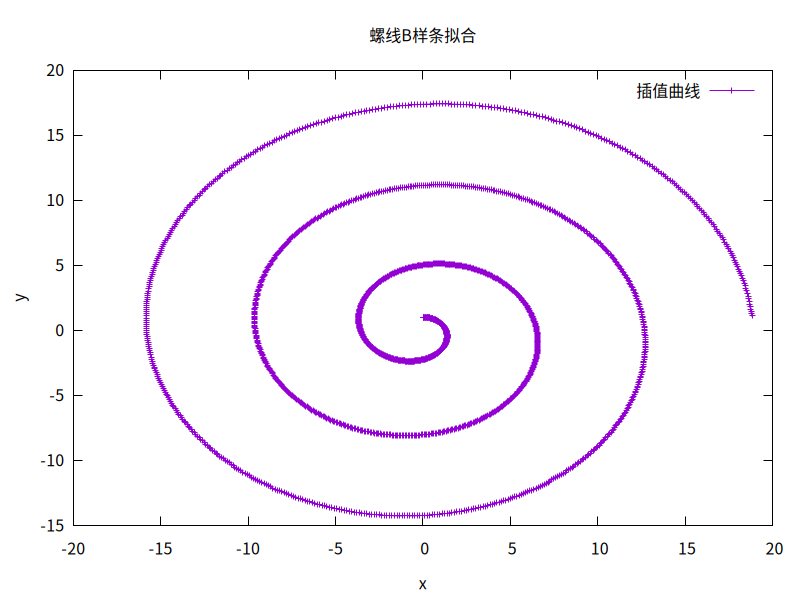
\includegraphics[scale=0.15]{../figure/FC160.png}
    \caption{N=10, N=40, N=160}
\end{figure}
\textbf{Periodic}
\begin{figure}[H]
    \centering
    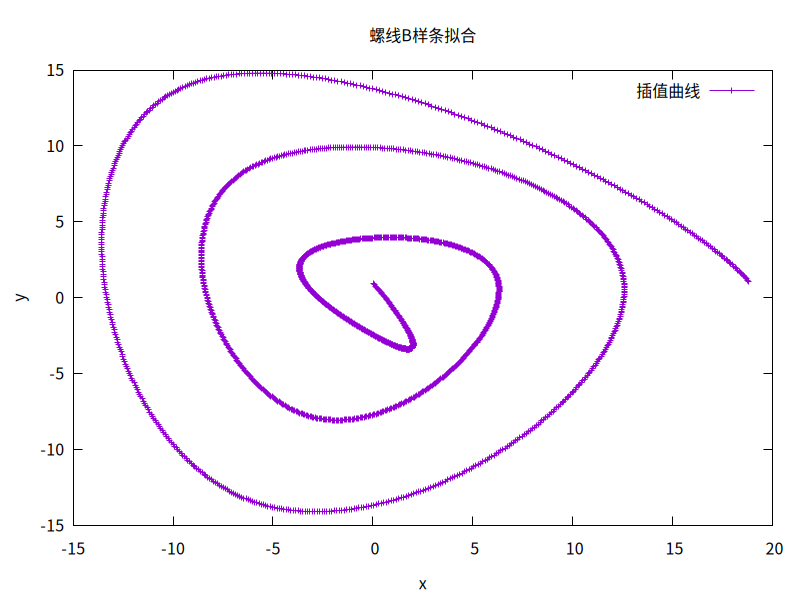
\includegraphics[scale=0.15]{../figure/FP10.png}
    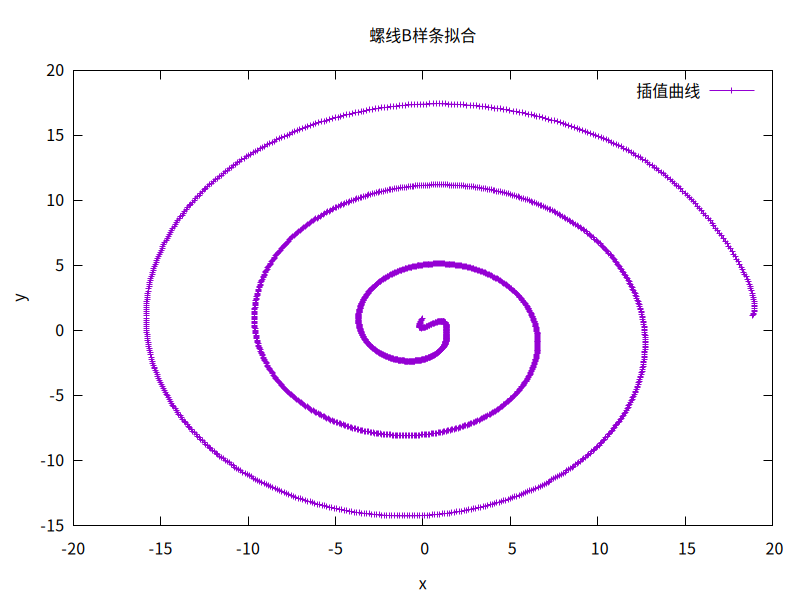
\includegraphics[scale=0.15]{../figure/FP40.png}
    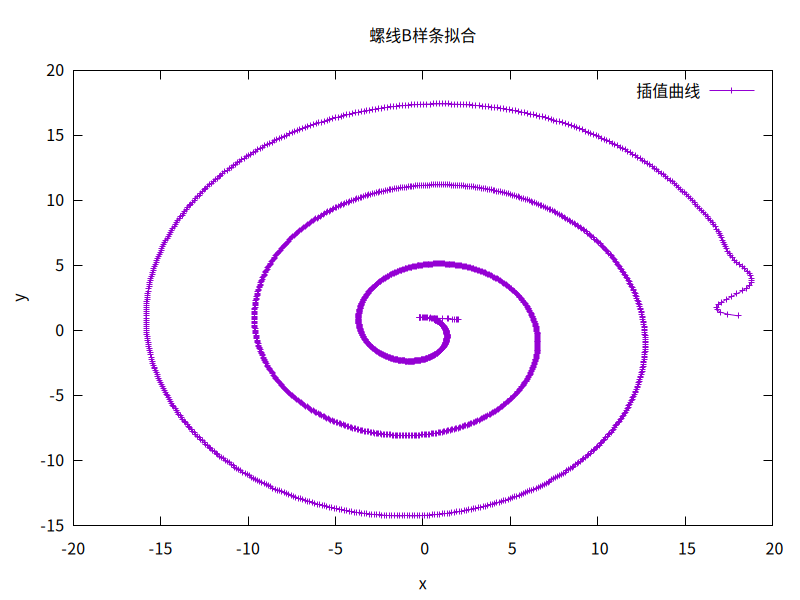
\includegraphics[scale=0.15]{../figure/FP160.png}
    \caption{N=10, N=40, N=160}
\end{figure}

Cumulative chordal length做法先求出函数在$[0, 6\pi]$的总长度，平均分成N段长度为h，
对每个h利用二分法求出对应的t值，再用t值计算插值函数的值。结果如下：
\textbf{Natural}
\begin{figure}[H]
    \centering
    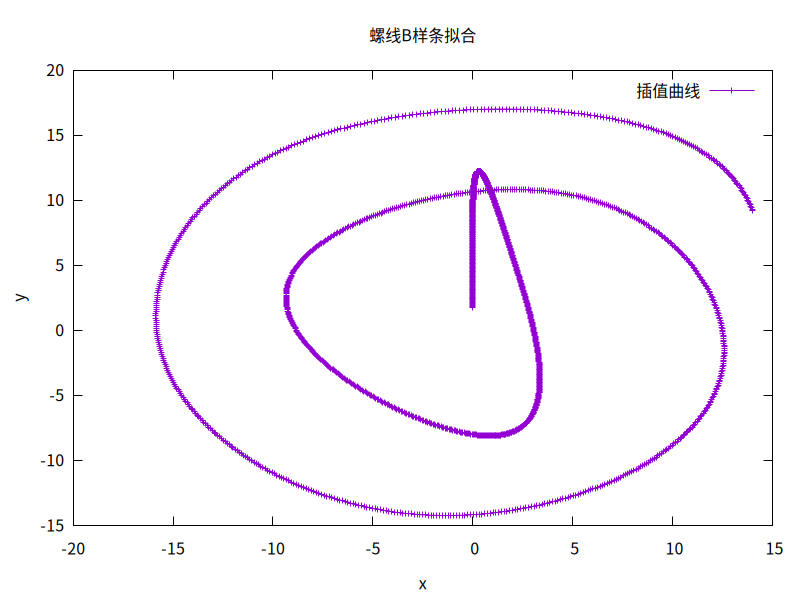
\includegraphics[scale=0.15]{../figure/FNC10.png}
    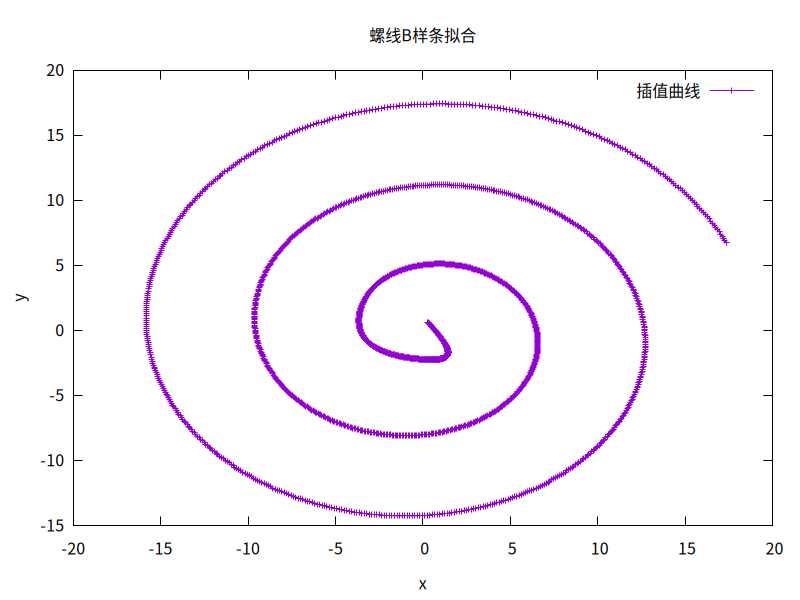
\includegraphics[scale=0.15]{../figure/FNC40.png}
    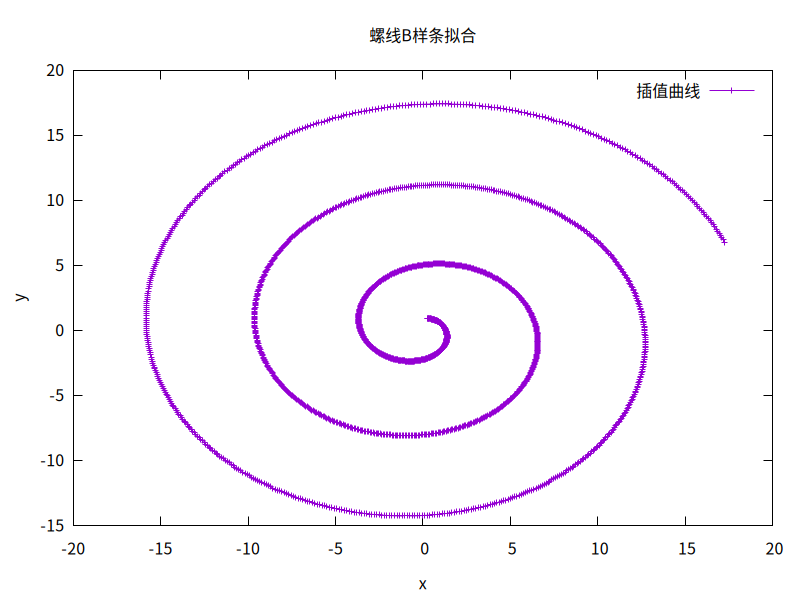
\includegraphics[scale=0.15]{../figure/FNC160.png}
    \caption{N=10, N=40, N=160}
\end{figure}
\textbf{Complete}
\begin{figure}[H]
    \centering
    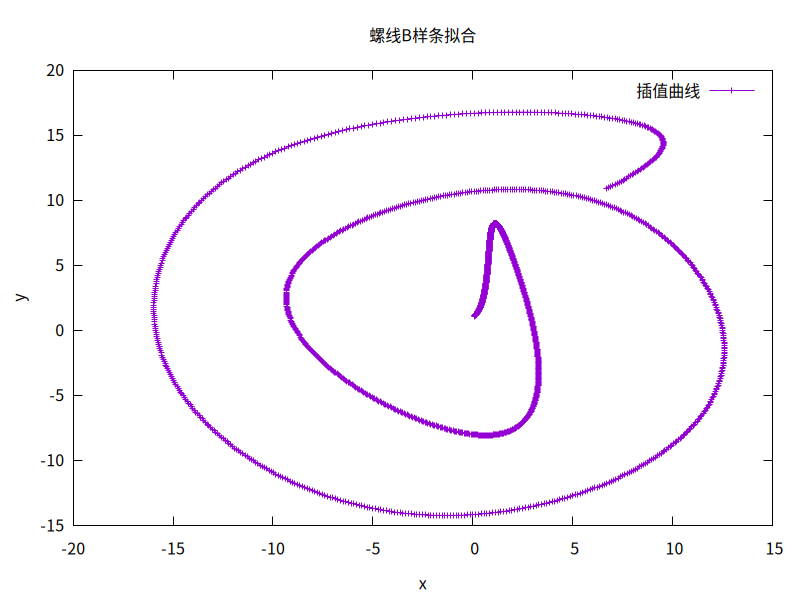
\includegraphics[scale=0.15]{../figure/FCC10.png}
    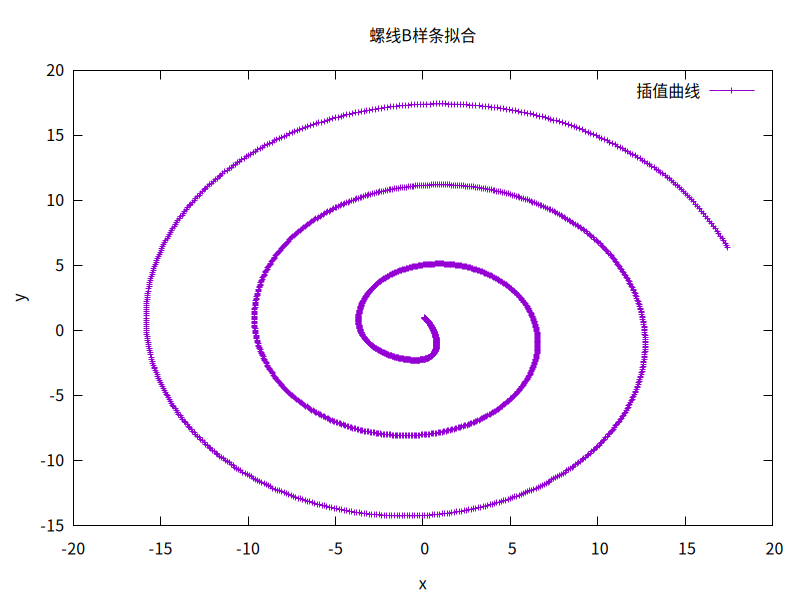
\includegraphics[scale=0.15]{../figure/FCC40.png}
    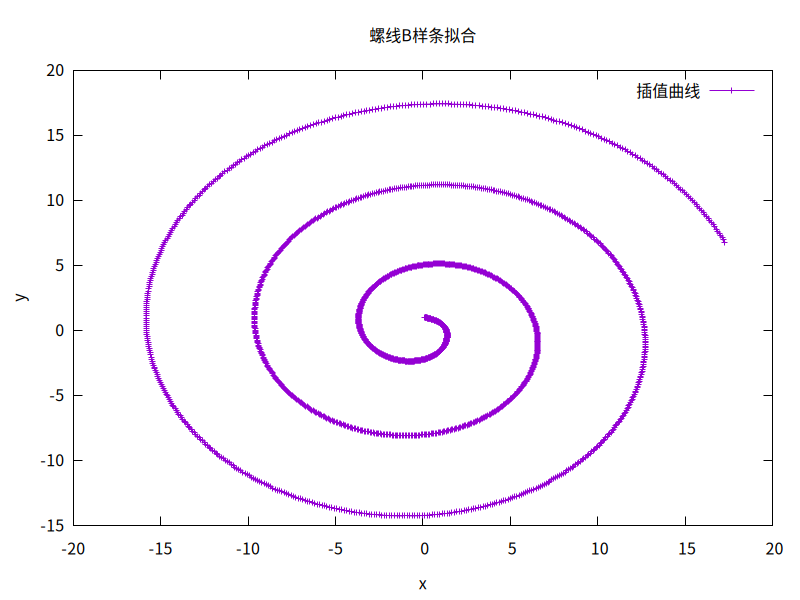
\includegraphics[scale=0.15]{../figure/FCC160.png}
    \caption{N=10, N=40, N=160}
\end{figure}
\textbf{Periodic}
\begin{figure}[H]
    \centering
    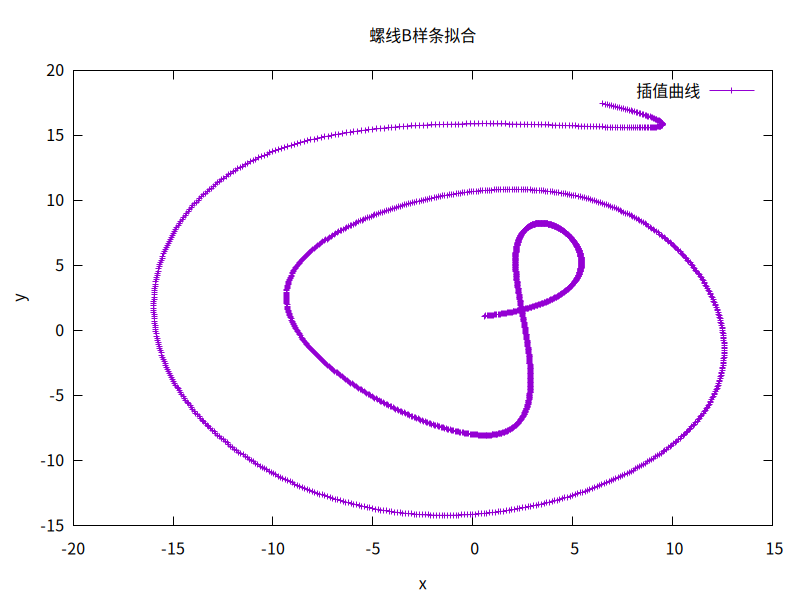
\includegraphics[scale=0.15]{../figure/FPC10.png}
    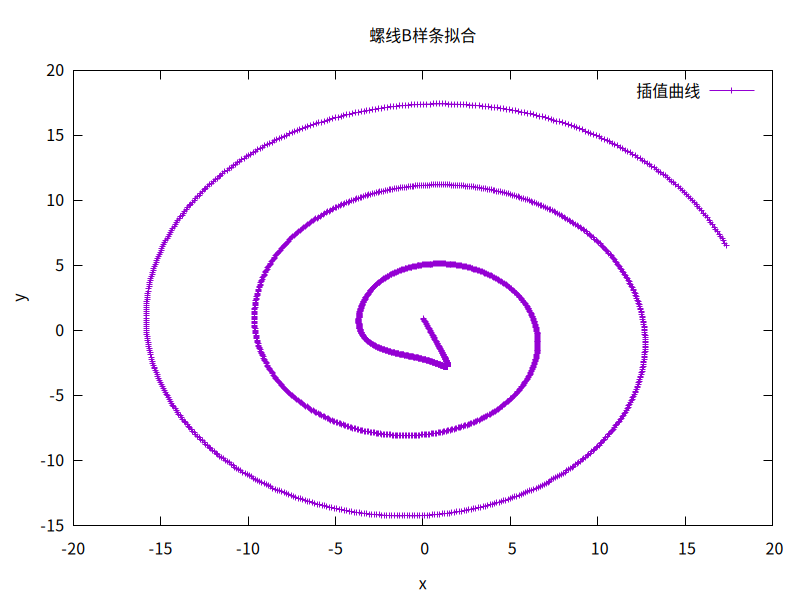
\includegraphics[scale=0.15]{../figure/FPC40.png}
    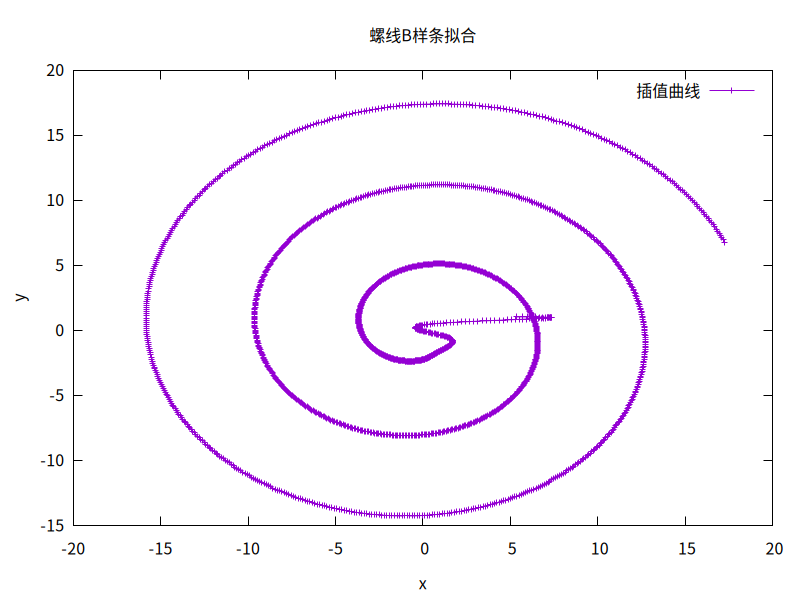
\includegraphics[scale=0.15]{../figure/FPC160.png}
    \caption{N=10, N=40, N=160}
\end{figure}

\subsection*{三维曲线}
\textbf{原图}
\begin{figure}[H]
    \centering
    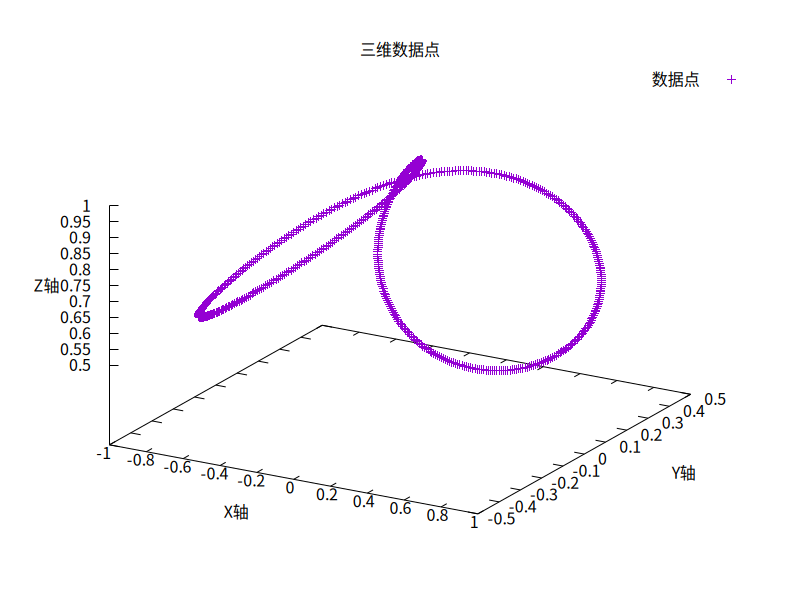
\includegraphics[scale=0.25]{../figure/G_real.png}
\end{figure}

因为求出弦长后发现$s(t) = t$,因此等距节点的结果就等于Cumulative chordal length的结果。

\textbf{Natural}
\begin{figure}[H]
    \centering
    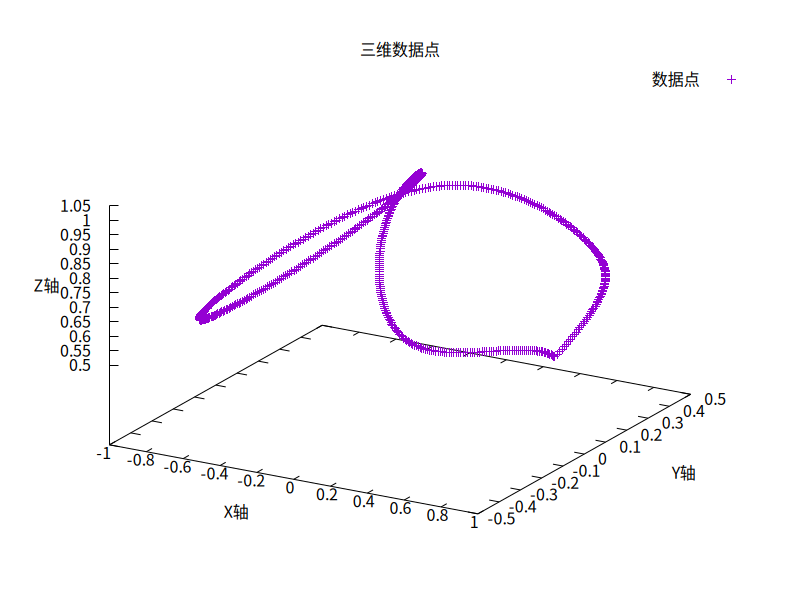
\includegraphics[scale=0.15]{../figure/GN10.png}
    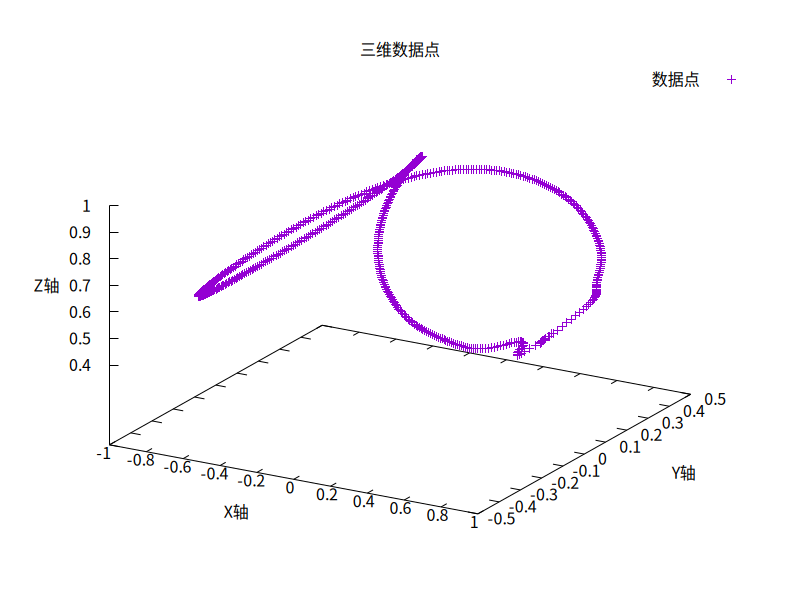
\includegraphics[scale=0.15]{../figure/GN40.png}
    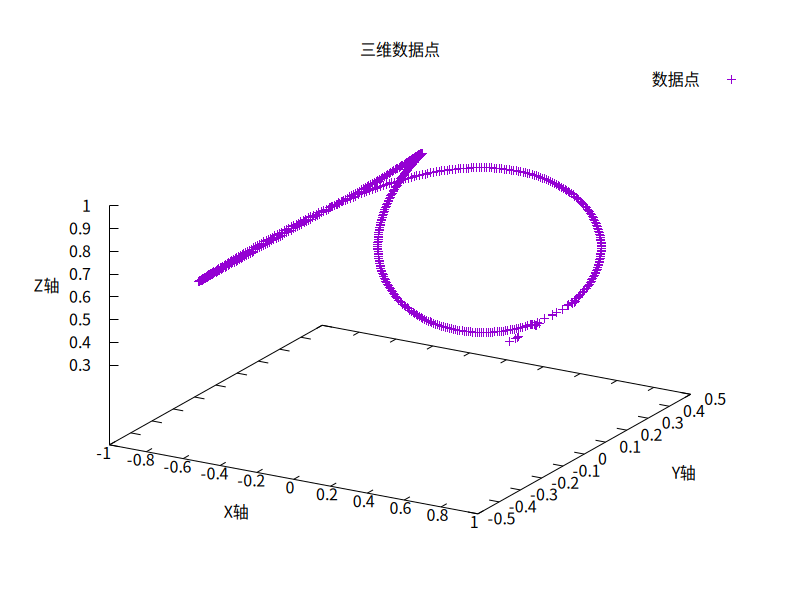
\includegraphics[scale=0.15]{../figure/GN160.png}
    \caption{N=10, N=40, N=160}
\end{figure}
\textbf{Complete}
\begin{figure}[H]
    \centering
    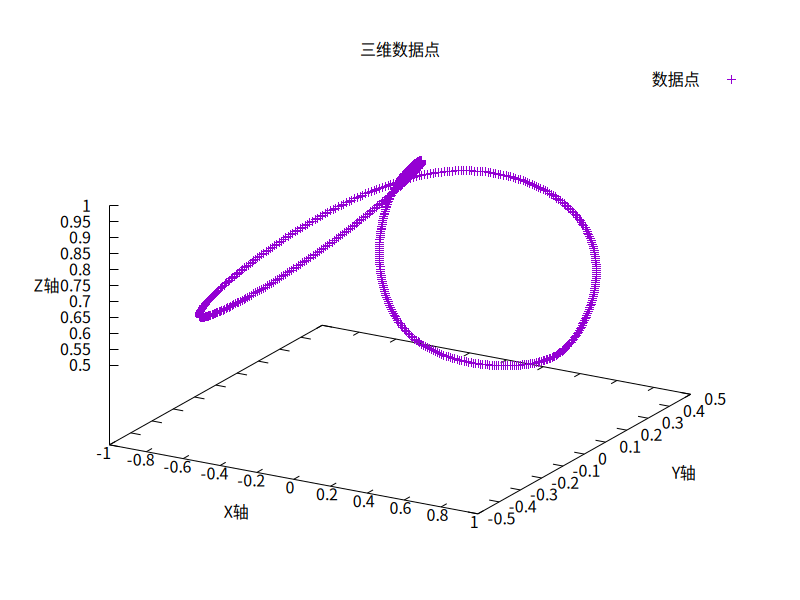
\includegraphics[scale=0.15]{../figure/GC10.png}
    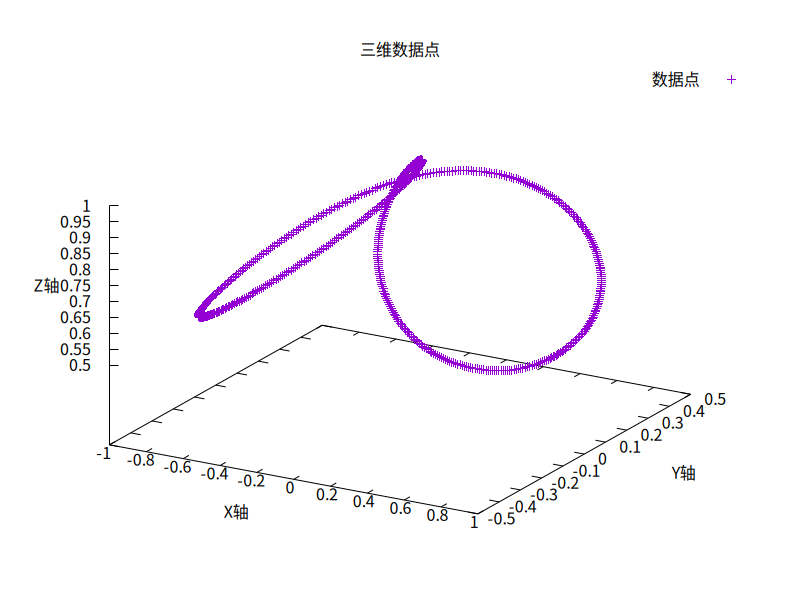
\includegraphics[scale=0.15]{../figure/GC40.png}
    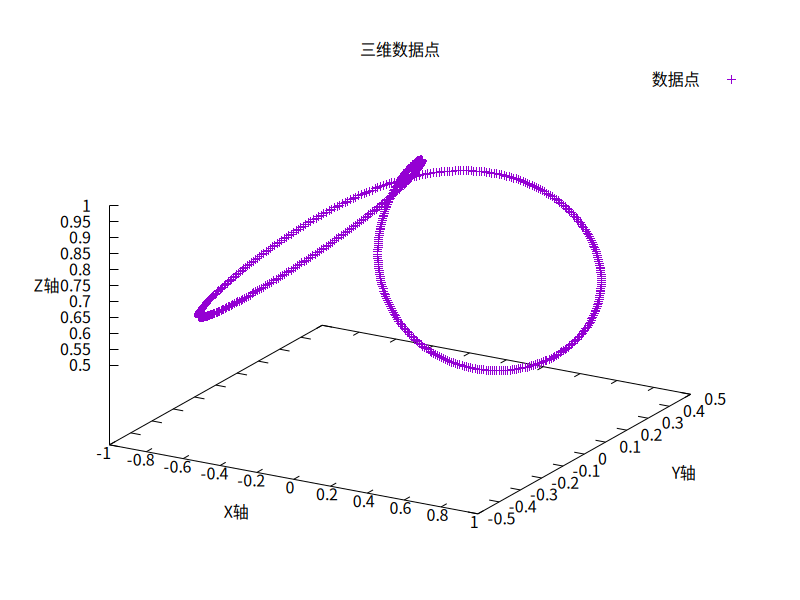
\includegraphics[scale=0.15]{../figure/GC160.png}
    \caption{N=10, N=40, N=160}
\end{figure}
\textbf{Periodic}
\begin{figure}[H]
    \centering
    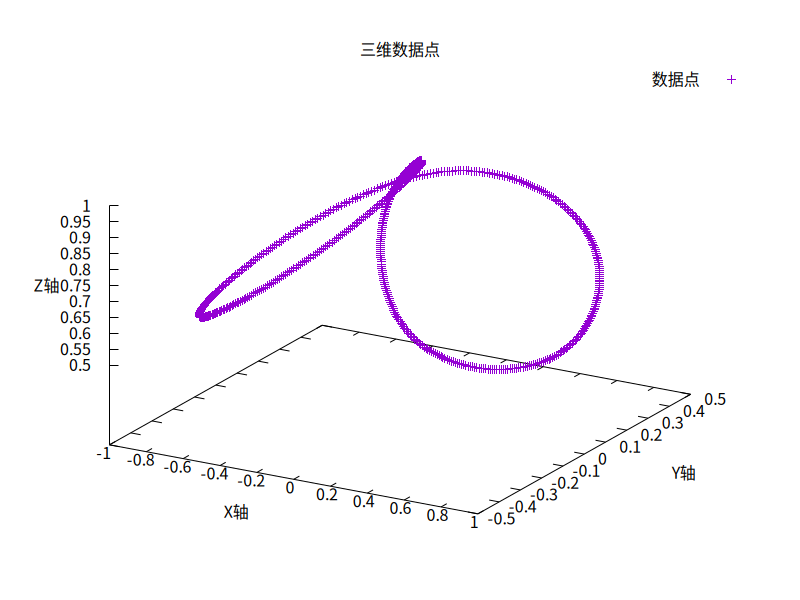
\includegraphics[scale=0.15]{../figure/GP10.png}
    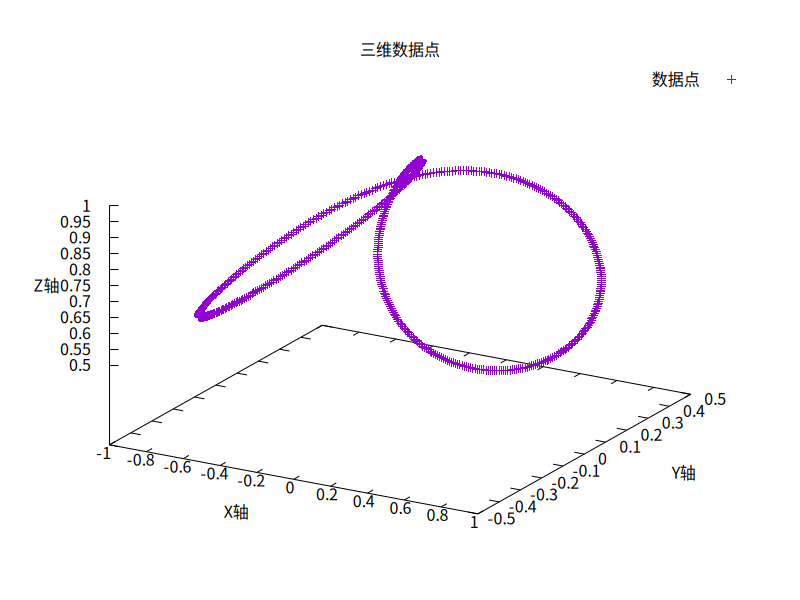
\includegraphics[scale=0.15]{../figure/GP40.png}
    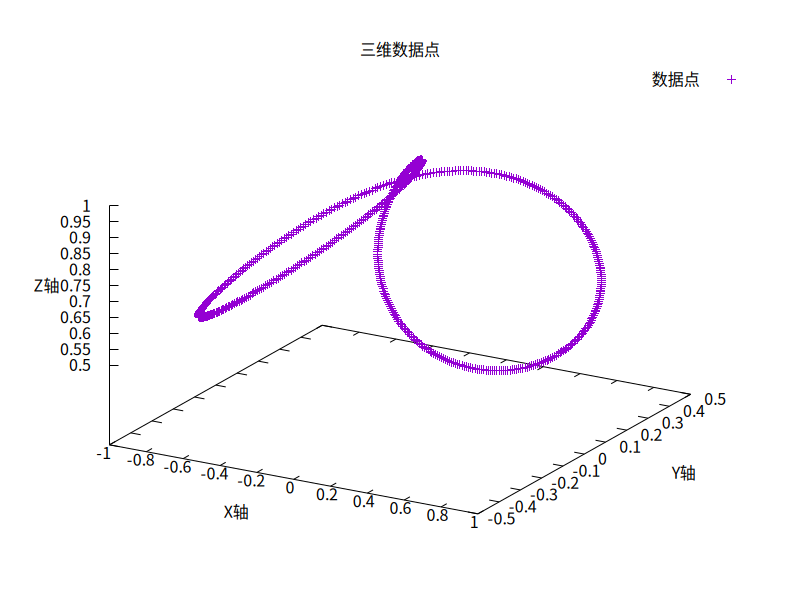
\includegraphics[scale=0.15]{../figure/GP160.png}
    \caption{N=10, N=40, N=160}
\end{figure}

\subsection*{更多例子}
\textbf{Sinx}
\begin{figure}[H]
    \centering
    \includegraphics[scale=0.3]{../figure/sinx.png}
\end{figure}

\textbf{$e^{x}$}
\begin{figure}[H]
    \centering
    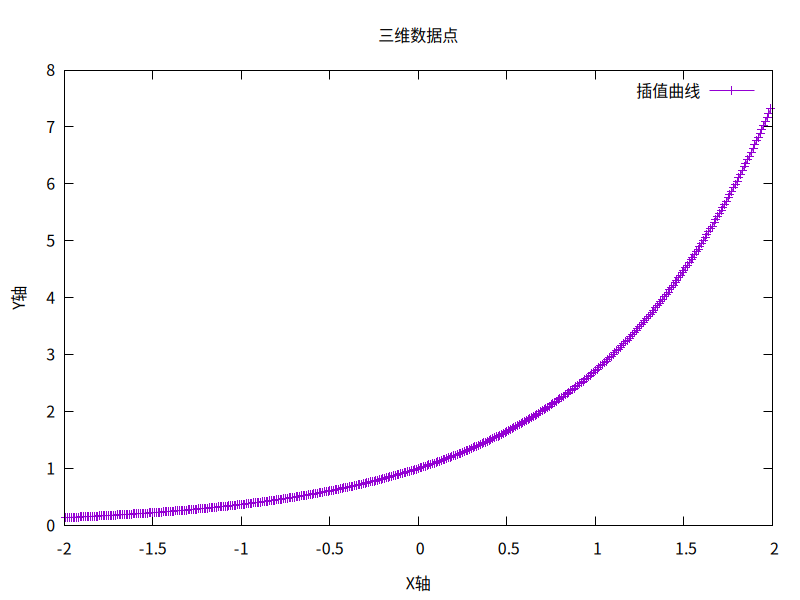
\includegraphics[scale=0.3]{../figure/ex.png}
\end{figure}

\textbf{$e^{x} \sin(x)$}
\begin{figure}[H]
    \centering
    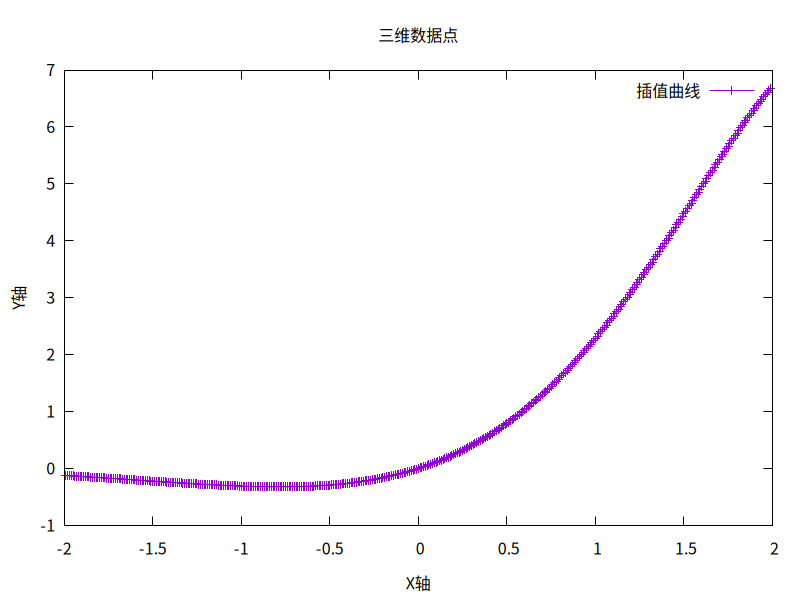
\includegraphics[scale=0.3]{../figure/expsinx.png}
\end{figure}

发现这些更多例子都能够良好拟合。


\subsection*{任意阶的样条}
因为当阶数增加之后边界条件也需要增加，我测试了七次样条，对函数$\frac{1}{1+x^{2}}$进行拟合结果如下：

\begin{figure}[H]
    \centering
    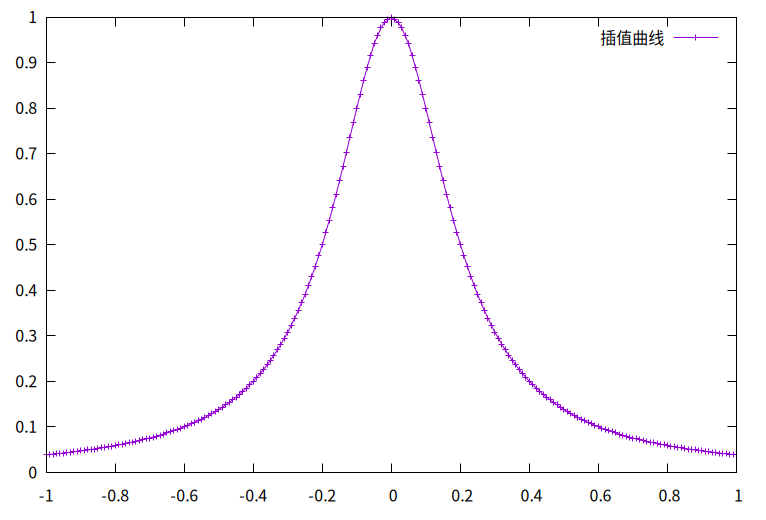
\includegraphics[scale=0.3]{../figure/SevenFit.png}
\end{figure}





\end{document}
